\documentclass{ctexart}

\usepackage{amsmath,amsthm,extarrows,color,enumitem}
\usepackage[a4paper, left = 1.5cm, right = 1.5cm]{geometry}
% 加载 geometry 并设置一个非常大的页面高度
% layoutwidth 可以根据需要调整，layoutheight 设置为一个极大的值
%\usepackage[
%    paperwidth=15cm, 
%    paperheight=500cm, % 设置一个足够长的值，例如 5 米
%    margin=1cm
%]{geometry}
%
%\pagestyle{empty} % 隐藏页码

\usepackage[hyperref=true,backend=biber,sorting=none,backref=true]{biblatex}
\DefineBibliographyStrings{english}{%
  backrefpage = {page},% originally "cited on page"
  backrefpages = {pages},% originally "cited on pages"
}

\usepackage{hyperref}
\hypersetup{
     colorlinks   = true,
     linkcolor=blue,
     citecolor=red,
     %filecolor=magenta,      % color of file links
     urlcolor=cyan
}
\usepackage{cleveref}
\usepackage{microtype}

\usepackage{listings}
\usepackage{xcolor}  % 颜色支持

% 基础配置
\lstset{
    basicstyle=\ttfamily\small,      % 等宽小字体
    keywordstyle=\color{blue},       % 关键字蓝色
    commentstyle=\color{gray},       % 注释灰色
    stringstyle=\color{red},         % 字符串红色
    numbers=left,                    % 行号在左
    numberstyle=\tiny\color{gray},
    frame=single,                    % 边框
    breaklines=true,                 % 自动换行
    showstringspaces=false,          % 不显示空格标记
}

\theoremstyle{remark}
\newtheorem*{remark}{备注}

% 1. 定义一个新的定理样式
\newtheoremstyle{warningstyle}
  {3pt}                % 上间距
  {3pt}                % 下间距
  {}                   % 文本字体 (默认罗马)
  {}                   % 缩进量
  {\bfseries}          % 标题字体
  {:}                  % 标题后符号
  {.5em}               % 标题与文本间距
  {}                   % 标题规格

% 2. 使用新样式定义环境
\theoremstyle{warningstyle}
\newtheorem*{warning}{警告} % * 表示不编号

\theoremstyle{warningstyle}
\newtheorem*{danger}{危险}


\setlength{\parindent}{0pt}

\usepackage{graphicx}
\graphicspath{{./images/}}

\usepackage{float}

\usepackage{array}
\usepackage{booktabs}

\usepackage{cprotect}

\title{亲手实现 Git！\footnote{\href{https://wyag.thb.lt/}{Write yourself a Git!}}}
\author{}
\date{}

\begin{document}
\maketitle
\section{简介}
\begin{remark}
近期更新（最后更新于 2026 年 4 月）：
\begin{itemize}
  \item 新增关于默克尔有向无环图（Merkle DAG）的理论讲解章节
  \item 本目录现已改为自动生成
\end{itemize}
\end{remark}

本文旨在从底层原理开始完整讲解 Git 版本控制系统，也就是从最基础的内核机制出发，逐层向上剖析。这件事听起来并不简单，前人也曾多次尝试讲解，但效果参差不齐。不过本文提供了一条简单易懂的路径：想要搞懂 Git 内部原理，最好的方式就是从零重新实现一遍 Git。

别着急划走。

这并非玩笑，而且整体逻辑并不复杂：只要你通读全文、亲手编写代码（当然你也可以直接\href{https://wyag.thb.lt/wyag.zip}{下载}源码压缩包，但真心建议自己动手敲代码），最终你会得到一个名为 wyag 的程序。它实现了 Git 全部核心基础功能：init、add、rm、status、commit、log 等，并且原生兼容原版 Git。兼容性极高，甚至本文中「提交章节」本身的那次提交，就是由你写出来的 wyag 完成，而非官方 Git。整套实现仅用 983 行简洁的 Python 代码 即可完成。

可 Git 本身这么复杂，真的适合从零复刻吗？在我看来，Git 很复杂其实是一种误解。诚然，Git 体量庞大、功能繁多，但它的核心原理其实极其简单。我们平时觉得它晦涩难懂，首先是因为它的设计思路常常与直觉相悖（网上那些五花八门的趣味比喻文章，反倒越解释越乱）。而真正让人困惑的根源，或许正是它核心模型极致的简洁与强大。底层原理极简，上层应用却极为丰富，这种反差会让人很难理解；你需要完成一次思维跨越，才能从最本质、最朴素的抽象模型，推导出各式各样复杂的上层功能（就像函数里的单子理论，懂的都懂）。

亲手实现一遍 Git，就能让它最底层的原理毫无保留地展现在你面前。

\textbf{你能学到什么?}
本文会详细实现并讲解一套精简版 Git 核心命令（但凡有讲解不清的地方，欢迎反馈指正）。代码会力求简洁直白，因此我们编写的 wyag 程序远达不到原版 Git 命令行的完整能力，但所有缺失的功能都十分浅显，愿意动手尝试的人都可以轻松补全。用业内的话说：将 wyag 升级为功能完备的 Git 库与命令行工具，留给读者自行拓展练习。
具体我们会实现以下命令：
  \begin{itemize}
    \item add
    \item cat-file
    \item check-ignore
    \item checkout
    \item commit
    \item hash-object
    \item init
    \item log
    \item ls-files
    \item ls-tree
    \item rev-parse
    \item rm
    \item show-ref
    \item status
    \item tag
  \end{itemize}
学习本文几乎不需要深厚基础，仅需掌握：基础 Git 用法、基础 Python 语法、基础 Shell 操作即可。
\begin{itemize}
    \item Git 方面：我默认你熟悉最基础的 Git 指令，无需精通。但如果你从未使用过 init、add、rm、commit、checkout 这类基础命令，阅读过程会非常吃力。
    \item 编程语言方面：wyag 全程使用 Python 编写。代码不会用到高阶语法，Python 本身可读性也接近伪代码，整体很好理解。有意思的是，全文最复杂的部分反而是命令行参数解析，这部分你就算不懂也完全不影响核心原理学习。如果你会编程但从未接触过 Python，建议在网上快速入门熟悉一下语法即可。
    \item 终端操作方面：wyag 和原版 Git 都是终端程序。我默认你会基础的类 Unix 终端操作，不用精通高阶技巧，但 cd、ls、rm、tree 这类基础命令需要熟练使用。
\end{itemize}
\begin{warning}
Windows 用户须知

wyag 可在所有搭载 Python 环境的类 Unix 系统上运行，但完全无法保证在原生 Windows 系统上正常运行。本项目的测试套件必须依赖兼容 bash 的终端环境，Windows 用户可使用 WSL（Windows 子系统）运行。若你使用 WSL，需确保 wyag 文件为 Unix 换行符格式（使用 VS Code 的用户可参考 Stack Overflow 相关解决方案）。非常欢迎 Windows 用户反馈运行问题！
\end{warning}
\begin{remark}
致谢

本文的完善离不开多位开发者的大量贡献，在此一并致谢。特别感谢：
\begin{itemize}
    \item GitHub 用户 tammoippen：最初编写了我遗漏的 \verb|tag_create| 标签创建函数（对应 Issue \verb|#9|）。
    \item GitHub 用户 hjlarry：修复了项目 \verb|#22| 中的多处问题。
    \item GitHub 用户 cutebbb：在 \verb|#32| 中实现了 ls-files 的初代版本，借此完善了 wyag 的暂存区功能！
    \item Manuel Pégourié-Gonnard：解开了树对象排序规则的谜题，并优化了 \verb|tree_leaf_sort_key| 排序函数。
\end{itemize}
\end{remark}

\section{入门准备}

你需要准备 Python 3.10 及以上版本，以及你常用的文本编辑器。本项目不需要任何第三方库、虚拟环境，除了原生 Python 解释器外无需额外依赖，所有用到的功能全部来自 Python 标准库。

我们会把代码拆分成两个文件：
\begin{itemize}
    \item 可执行程序文件：wyag
    \item Python 库文件：libwyag.py
\end{itemize}
所有软件项目开头都免不了一堆模板化初始化代码，我们先把这部分搞定。

首先创建简短的可执行文件。在编辑器中新建名为 wyag 的文件，粘贴下面几行代码：
\begin{lstlisting}[language=Python]
#!/usr/bin/env python3

import libwyag
libwyag.main()
\end{lstlisting}
然后赋予该文件可执行权限：
\begin{lstlisting}[language=bash]
$ chmod +x wyag
\end{lstlisting}
到这里就完成了！

接下来编写库文件。该文件必须命名为 libwyag.py，并且和 wyag 可执行文件放在同一个目录下。先在编辑器中新建空白的 libwyag.py。

首先需要导入一系列模块（直接完整复制即可）：
\begin{itemize}
\item Git 是命令行工具，因此我们需要解析命令行参数。Python 内置的 argparse 模块可以帮我们完成绝大部分相关工作。
\begin{lstlisting}[language=Python]
import argparse
\end{lstlisting}
\item Git 的配置文件采用类似微软 INI 的格式，configparser 模块可以实现这类文件的读写。
\begin{lstlisting}[language=Python]
import configparser
\end{lstlisting}
\item 我们需要处理日期与时间相关操作：
\begin{lstlisting}[language=Python]
from datetime import datetime
\end{lstlisting}
\item 后续需要读取类 Unix 系统下的用户与用户组信息（grp 对应用户组，pwd 对应用户）。因为 Git 会存储文件所属用户、用户组的数字 ID，我们需要把这些 ID 转换成易读的文字展示；Windows 系统没有这两个模块，因此做异常兼容处理。
\begin{lstlisting}[language=Python]
try:
    import grp, pwd
except ModuleNotFoundError:
    pass
\end{lstlisting}
\item 为了实现 .gitignore 忽略文件功能，需要用通配符匹配文件名，fnmatch 模块专门处理这类匹配：
\begin{lstlisting}[language=Python]
from fnmatch import fnmatch
\end{lstlisting}
\item Git 大量使用 SHA-1 哈希算法，Python 中对应的模块为 hashlib：
\begin{lstlisting}[language=Python]
import hashlib
\end{lstlisting}
\item 引入数学模块中的向上取整函数：
\begin{lstlisting}[language=Python]
from math import ceil
\end{lstlisting}
\item os 与 os.path 模块提供文件系统相关的基础操作接口：
\begin{lstlisting}[language=Python]
import os
\end{lstlisting}
\item 我们会用到少量正则表达式功能：
\begin{lstlisting}[language=Python]
import re
\end{lstlisting}
\item sys 模块用于获取原始命令行参数（sys.argv）：
\begin{lstlisting}[language=Python]
import sys
\end{lstlisting}
\item Git 内部所有对象都会通过 zlib 压缩，Python 内置了该压缩模块：
\begin{lstlisting}[language=Python]
import zlib
\end{lstlisting}
\end{itemize}
模块导入部分完成。项目会频繁处理命令行参数，Python 的 argparse 库简单且功能够用。这个库本身很不错，只是接口设计不算直观，有需要可以查阅官方文档。
\begin{lstlisting}[language=Python]
argparser = argparse.ArgumentParser(description="The stupidest content tracker")
\end{lstlisting}
Git 采用子命令模式（比如 git init、git commit），在 argparse 中这类功能叫做子解析器。我们先声明程序支持子命令，并且运行时必须传入子命令—— 你不能只输入 git，必须输入 git COMMAND。
\begin{lstlisting}[language=Python]
argsubparsers = argparser.add_subparsers(title="Commands", dest="command")
argsubparsers.required = True
\end{lstlisting}
参数 dest="command" 表示：用户输入的子命令名称，会以字符串形式存入 command 字段。之后我们只需要读取这个字符串，调用对应的功能函数即可。按照规范，我把这些转接函数统一称为桥接函数，命名全部以 \verb|cmd_| 开头。桥接函数接收解析后的参数作为唯一入参，负责参数校验、预处理，再调用真正的功能逻辑。
\begin{lstlisting}[language=Python]
def main(argv=sys.argv[1:]):
    args = argparser.parse_args(argv)
    match args.command:
        case "add"          : cmd_add(args)
        case "cat-file"     : cmd_cat_file(args)
        case "check-ignore" : cmd_check_ignore(args)
        case "checkout"     : cmd_checkout(args)
        case "commit"       : cmd_commit(args)
        case "hash-object"  : cmd_hash_object(args)
        case "init"         : cmd_init(args)
        case "log"          : cmd_log(args)
        case "ls-files"     : cmd_ls_files(args)
        case "ls-tree"      : cmd_ls_tree(args)
        case "rev-parse"    : cmd_rev_parse(args)
        case "rm"           : cmd_rm(args)
        case "show-ref"     : cmd_show_ref(args)
        case "status"       : cmd_status(args)
        case "tag"          : cmd_tag(args)
        case _              : print("Bad command.")
\end{lstlisting}

\section{创建仓库：init 命令}
无论是时间顺序还是逻辑顺序，Git 的第一个命令都是 git init，因此我们从实现 wyag init 开始。要完成这个功能，首先需要对仓库进行最基础的抽象封装。
\subsection{仓库对象}
我们必须对仓库进行抽象封装：几乎每次执行 Git 命令，都是在对仓库执行操作 —— 创建、读取或修改。
一个 Git 仓库由两部分组成：
\begin{itemize}
    \item 工作区（work tree）：存放需要被版本控制的文件
    \item Git 目录（git directory）：Git 存储自身数据的目录
\end{itemize}
绝大多数情况下，工作区就是一个普通文件夹，Git 目录是工作区下名为 .git 的子目录。

Git 支持更多场景（裸仓库、分离的 Git 目录等），但我们无需实现这些，只保留最基础的 worktree/.git 结构即可。我们的仓库对象仅存储两个路径：工作区路径和 Git 目录路径。

创建新的仓库(Repository)对象时，只需做几项校验：
\begin{itemize}
    \item 校验目录存在，且包含名为 .git 的子目录
    \item 读取 \lstinline|.git/config| 配置文件（标准 INI 格式），校验 \verb|core.repositoryformatversion| 的值为 0（后文会详细说明该字段）
\end{itemize}
构造函数包含一个可选的 \verb|force| 参数，用于禁用所有校验。这是因为我们后续实现的 \verb|repo_create()| 函数需要用仓库对象来创建仓库，因此需要支持在无效的文件系统路径下创建仓库对象。
\begin{lstlisting}[language=Python]
class GitRepository (object):
    """A git repository"""

    worktree = None
    gitdir = None
    conf = None

    def __init__(self, path, force=False):
        self.worktree = path
        self.gitdir = os.path.join(path, ".git")

        if not (force or os.path.isdir(self.gitdir)):
            raise Exception(f"Not a Git repository {path}")

        # Read configuration file in .git/config
        self.conf = configparser.ConfigParser()
        cf = repo_file(self, "config")

        if cf and os.path.exists(cf):
            self.conf.read([cf])
        elif not force:
            raise Exception("Configuration file missing")

        if not force:
            vers = int(self.conf.get("core", "repositoryformatversion"))
            if vers != 0:
                raise Exception(f"Unsupported repositoryformatversion: {vers}")
\end{lstlisting}
我们需要频繁操作仓库内的路径，因此封装几个工具函数来计算路径、自动创建缺失的目录结构。首先是基础的路径拼接函数：
\begin{lstlisting}[language=Python]
def repo_path(repo, *path):
    """Compute path under repo's gitdir."""
    return os.path.join(repo.gitdir, *path)
\end{lstlisting}
(Python 语法说明：\verb|*path| 表示可变参数，函数可以接收多个路径片段作为独立参数。示例：\lstinline|repo_path(repo, "objects", "df", "4ec9fc2ad990cb9da906a95a6eda6627d7b7b0")| 是合法调用，函数内部会将参数 \verb|path| 转为列表处理)

接下来两个函数 \verb|repo_file()| 和 \verb|repo_dir()| 分别用于获取文件/目录路径，并支持自动创建缺失的目录。区别在于：文件版本只会创建到最后一个组件之前的目录。
\begin{lstlisting}[language=Python]
def repo_file(repo, *path, mkdir=False):
    """Same as repo_path, but create dirname(*path) if absent.  For
example, repo_file(r, \"refs\", \"remotes\", \"origin\", \"HEAD\") will create
.git/refs/remotes/origin."""

    if repo_dir(repo, *path[:-1], mkdir=mkdir):
        return repo_path(repo, *path)

def repo_dir(repo, *path, mkdir=False):
    """Same as repo_path, but mkdir *path if absent if mkdir."""

    path = repo_path(repo, *path)

    if os.path.exists(path):
        if (os.path.isdir(path)):
            return path
        else:
            raise Exception(f"Not a directory {path}")

    if mkdir:
        os.makedirs(path)
        return path
    else:
        return None
\end{lstlisting}
语法说明：由于 \verb|*path| 是可变参数，\verb|mkdir| 必须显式指定参数名传递。示例：\lstinline|repo_file(repo, "objects", mkdir=True)|

要创建一个新的仓库，我们首先准备一个目录（如果该目录不存在则创建它），然后在该目录内部创建 Git 目录（该目录必须不存在，或者是空的）。这个目录名为 .git（在 Unix 系统上，开头的点表示它是“隐藏”目录），其中包含：
\begin{itemize}
\item \lstinline|.git/objects/|：对象存储区，我们将在下一节中介绍。
\item \lstinline|.git/refs/|：引用存储区，我们稍后会讨论。它包含两个子目录：heads 和 tags。
\item \lstinline|.git/HEAD|：一个指向当前 HEAD 的引用（更多内容将在后面介绍！）。
\item \lstinline|.git/config|：仓库的配置文件。
\item \lstinline|.git/description|：存放一个供人类阅读的、对该仓库内容的自由格式描述，通常很少使用。
\end{itemize}
\begin{lstlisting}[language=Python]
def repo_create(path):
    """Create a new repository at path."""

    repo = GitRepository(path, True)

    # First, we make sure the path either doesn't exist or is an
    # empty dir.

    if os.path.exists(repo.worktree):
        if not os.path.isdir(repo.worktree):
            raise Exception (f"{path} is not a directory!")
        if os.path.exists(repo.gitdir) and os.listdir(repo.gitdir):
            raise Exception (f"{path} is not empty!")
    else:
        os.makedirs(repo.worktree)

    assert repo_dir(repo, "branches", mkdir=True)
    assert repo_dir(repo, "objects", mkdir=True)
    assert repo_dir(repo, "refs", "tags", mkdir=True)
    assert repo_dir(repo, "refs", "heads", mkdir=True)

    # .git/description
    with open(repo_file(repo, "description"), "w") as f:
        f.write("Unnamed repository; edit this file 'description' to name the repository.\n")

    # .git/HEAD
    with open(repo_file(repo, "HEAD"), "w") as f:
        f.write("ref: refs/heads/master\n")

    with open(repo_file(repo, "config"), "w") as f:
        config = repo_default_config()
        config.write(f)

    return repo
\end{lstlisting}
配置文件非常简单，它是一个类似 INI 格式的文件，包含一个单独的段（\verb|[core]|）和三个字段：
\begin{itemize}
    \item \verb|repositoryformatversion = 0|：Git 目录格式的版本。0 表示初始格式，1 表示带有扩展的相同格式。如果大于 1，Git 会报错并退出；wyag 只接受 0。
    \item \verb|filemode = false|：禁用对工作树中文件模式（权限）变更的跟踪。
    \item \verb|bare = false|：表示该仓库包含一个工作树。Git 支持一个可选的 worktree 键，用于指定工作树的位置（如果不是 ..）；wyag 不支持此键。
\end{itemize}
我们使用 Python 的 configparser 库来创建这个文件：
\begin{lstlisting}[language=Python]
def repo_default_config():
    ret = configparser.ConfigParser()

    ret.add_section("core")
    ret.set("core", "repositoryformatversion", "0")
    ret.set("core", "filemode", "false")
    ret.set("core", "bare", "false")

    return ret
\end{lstlisting}

\cprotect\subsection{\verb|init| 命令}
现在我们有了读取和创建仓库的代码，让我们通过创建 wyag init 命令来使这些代码可以从命令行使用。wyag init 的行为类似于 git init——当然，可定制性要少得多。wyag init 的语法如下：
\begin{lstlisting}[language=bash]
wyag init [path]
\end{lstlisting}
我们已经拥有了完整的仓库创建逻辑。要创建这个命令，我们只需要两样东西：
\begin{enumerate}
    \item 我们需要创建一个 argparse 子解析器来处理命令的参数：
\begin{lstlisting}[language=Python]
argsp = argsubparsers.add_parser("init", help="Initialize a new, empty repository.")
\end{lstlisting}
对于 init 命令，有一个可选的、位置参数：要初始化仓库的路径。默认为 .，即当前目录：
\begin{lstlisting}[language=Python]
argsp.add_argument("path",
                   metavar="directory",
                   nargs="?",
                   default=".",
                   help="Where to create the repository.")
\end{lstlisting}
\item 我们还需要一个“桥接”函数，从 argparse 返回的对象中读取参数值，并用正确的值调用实际的函数：
\begin{lstlisting}[language=Python]
def cmd_init(args):
    repo_create(args.path)
\end{lstlisting}
\end{enumerate}
大功告成！如果你按照这些步骤操作，现在你应该能够在任何地方使用 wyag init 初始化一个 Git 仓库：
\begin{lstlisting}[language=bash]
$ wyag init test
\end{lstlisting}
（注意：wyag 可执行文件通常不在你的 \$PATH 中——你需要使用完整路径来调用它，例如 \lstinline|~/projects/wyag/wyag init .|）

\cprotect\subsection{\verb|repo_find()| 函数}
在实现仓库功能的过程中，我们需要一个函数来查找当前仓库的根目录。我们会经常使用它，因为几乎所有的 Git 函数都是在一个已存在的仓库上工作的（当然，除了 init 命令！）。有时这个根目录就是当前目录，但也可能是父目录：你的仓库根目录可能在 \lstinline|~/Documents/MyProject|，但你可能正在 \lstinline|~/Documents/MyProject/src/tui/frames/mainview/| 目录下工作。

我们现在要创建的 \lstinline|repo_find()| 函数将从当前目录开始，递归向上回溯到 / 目录，来查找这个根目录。为了将一个路径识别为仓库，它会检查该路径下是否存在 .git 目录。
\begin{lstlisting}[language=Python]
def repo_find(path=".", required=True):
    path = os.path.realpath(path)

    if os.path.isdir(os.path.join(path, ".git")):
        return GitRepository(path)

    # If we haven't returned, recurse in parent, if w
    parent = os.path.realpath(os.path.join(path, ".."))

    if parent == path:
        # Bottom case
        # os.path.join("/", "..") == "/":
        # If parent==path, then path is root.
        if required:
            raise Exception("No git directory.")
        else:
            return None

    # Recursive case
    return repo_find(parent, required)
\end{lstlisting}
仓库相关的工作就完成了！

\section{读取和写入对象：hash-object 和 cat-file}
\subsection{什么是对象？}
现在我们有了仓库，接下来就该向仓库中存放东西了。而且，仅仅通过一堆 \texttt{mkdir} 来实现 Git 是无聊的。让我们来谈谈对象，并实现 \texttt{git hash-object} 和 \texttt{git cat-file}。

也许你不太熟悉这两个命令——它们并不是日常 Git 工具箱中的常用命令，实际上它们是相当底层的命令（用 Git 的说法是``管道命令"）。它们的功能其实非常简单：hash-object 将现有文件转换为 Git 对象，而 cat-file 则将现有的 Git 对象打印到标准输出。

那么，Git 对象究竟是什么？从核心上讲，Git 是一个``内容寻址的文件系统"。这意味着，与普通文件系统中文件名是任意的且与文件内容无关不同，Git 存储的文件名是通过数学方法从文件内容推导出来的。这有一个非常重要的含义：如果一个文本文件的单个字节发生了变化，它的内部名称也会随之改变。简单来说：在 Git 中你不会修改一个文件，而是在不同的位置创建一个新文件。对象就是这样：Git 仓库中的文件，其路径由它们的内容决定。

\begin{warning}
Git 并不（完全）是键值存储

一些文档，包括优秀的《Pro Git》，将 Git 称为``键值存储"。这并不算错，但可能会引起误解。实际上，普通文件系统比 Git 更接近键值存储。因为 Git 是从数据计算键值的，更准确地应该称之为``值-值存储"。
\end{warning}
Git 使用对象来存储很多东西：首先也是最重要的，是它进行版本控制的实际文件——例如源代码。提交（commit）也是对象，标签（tag）也是。除了少数明显的例外（我们稍后会看到！），在 Git 中几乎所有的东西都是作为对象存储的。

Git 存储给定对象的路径是通过计算其内容的 SHA-1 哈希值来确定的。更精确地说，Git 将哈希值呈现为小写的十六进制字符串，并将其分成两部分：前两个字符和剩余部分。它使用第一部分作为目录名，剩余部分作为文件名（这是因为大多数文件系统不喜欢单个目录中有太多文件，否则会慢如蜗牛。Git 的方法创建了 256 个可能的中间目录，从而将每个目录的平均文件数除以 256）。

\begin{remark}
什么是哈希函数？

SHA-1 就是我们所说的``哈希函数"。简单来说，哈希函数是一种单向数学函数：计算一个值的哈希很容易，但无法反向计算出哪个值产生了这个哈希。

哈希函数一个非常简单的例子是经典的 len（或 strlen）函数，它返回字符串的长度。计算字符串的长度非常容易，给定字符串的长度永远不会改变（当然，除非字符串本身发生变化！），但仅凭长度是不可能恢复原始字符串的。加密哈希函数是更复杂的版本，其附加属性是：计算一个能够产生给定哈希的输入非常困难，以至于实际上不可能做到。（要产生一个满足 \lstinline|strlen(i) == 12| 的输入 i，你只需输入 12 个随机字符。但对于 SHA-1 这样的算法，这将花费非常非常长的时间——长到实际上不可能实现\footnote{你或许已经知道，SHA-1 的碰撞已被发现。实际上，Git 已经不再使用原始的 SHA-1 了：它采用了一种加固的变体，虽然并非标准 SHA 算法，但除了那两个已知能产生碰撞的 PDF 文件外，它对所有其他已知输入都会产生相同的哈希值。}。）
\end{remark}
在我们开始实现对象存储系统之前，必须理解其确切的存储格式。一个对象以一个指定其类型的头部开始：blob、commit、tag 或 tree（稍后会详细介绍）。这个头部后面跟着一个 ASCII 空格（0x20），然后是对象大小（以 ASCII 数字表示的字节数），接着是空字节（0x00），最后是对象的内容。在 Wyag 仓库中，一个提交对象的前 48 个字节看起来像这样：
\begin{lstlisting}[language=bash]
00000000  63 6f 6d 6d 69 74 20 31  30 38 36 00 74 72 65 65  |commit 1086.tree|
00000010  20 32 39 66 66 31 36 63  39 63 31 34 65 32 36 35  | 29ff16c9c14e265|
00000020  32 62 32 32 66 38 62 37  38 62 62 30 38 61 35 61  |2b22f8b78bb08a5a|
\end{lstlisting}
在第一行中，我们看到类型头部、一个空格（0x20）、ASCII 格式的大小（1086）和空字节分隔符 0x00。第一行最后四个字节是该对象内容的开始，即单词``tree"——我们将在讨论提交时进一步讨论。

对象（头部和内容）使用 zlib 压缩存储。

\subsection{通用的对象基类}
对象可以有多种类型，但它们都共享相同的存储/检索机制和相同的通用头部格式。在深入探讨各种类型对象的细节之前，我们需要对这些共同特征进行抽象。最简单的方法是创建一个通用的 GitObject 基类，其中包含两个未实现的方法：\lstinline|serialize()| 和 \lstinline|deserialize()|，以及一个默认的 init() 方法，用于在需要时创建一个新的空对象（抱歉，Python 爱好者们，这不是很优雅的设计，但可能比复杂的构造函数更容易理解）。我们的 \lstinline|__init__| 方法要么从提供的数据中加载对象，要么调用子类提供的 init() 方法来创建一个新的空对象。

稍后，我们将继承这个通用类，为每种对象格式实际实现这些函数。
\begin{lstlisting}[language=Python]
class GitObject (object):

    def __init__(self, data=None):
        if data != None:
            self.deserialize(data)
        else:
            self.init()

    def serialize(self, repo):
        """This function MUST be implemented by subclasses.

It must read the object's contents from self.data, a byte string, and
do whatever it takes to convert it into a meaningful representation.
What exactly that means depend on each subclass.

        """
        raise Exception("Unimplemented!")

    def deserialize(self, data):
        raise Exception("Unimplemented!")

    def init(self):
        pass # Just do nothing. This is a reasonable default!
\end{lstlisting}

\subsection{读取对象}
要读取一个对象，我们需要知道它的 SHA-1 哈希值。然后根据这个哈希值计算其路径（使用上面解释的公式：前两个字符，然后是目录分隔符 /，再然后是剩余部分），并在 git 目录下的 objects 目录中查找它。也就是说，\lstinline|e673d1b7eaa0aa01b5bc2442d570a765bdaae751| 的路径是 \lstinline|.git/objects/e6/73d1b7eaa0aa01b5bc2442d570a765bdaae751|。

然后，我们将该文件作为二进制文件读取，并使用 zlib 解压缩。

从解压后的数据中，我们提取两个头部组件：对象类型和对象大小。根据类型，我们确定要使用的实际类。我们将大小转换为 Python 整数，并检查是否匹配。

一切完成后，我们只需调用该对象格式的正确构造函数。
\begin{lstlisting}[language=Python]
def object_read(repo, sha):
    """Read object sha from Git repository repo.  Return a
    GitObject whose exact type depends on the object."""

    path = repo_file(repo, "objects", sha[0:2], sha[2:])

    if not os.path.isfile(path):
        return None

    with open (path, "rb") as f:
        raw = zlib.decompress(f.read())

        # Read object type
        x = raw.find(b' ')
        fmt = raw[0:x]

        # Read and validate object size
        y = raw.find(b'\x00', x)
        size = int(raw[x:y].decode("ascii"))
        if size != len(raw)-y-1:
            raise Exception(f"Malformed object {sha}: bad length")

        # Pick constructor
        match fmt:
            case b'commit' : c=GitCommit
            case b'tree'   : c=GitTree
            case b'tag'    : c=GitTag
            case b'blob'   : c=GitBlob
            case _:
                raise Exception(f"Unknown type {fmt.decode('ascii')} for object {sha}")

        # Call constructor and return object
        return c(raw[y+1:])
\end{lstlisting}

\subsection{写入对象}
写入对象的过程与读取相反：我们计算哈希值，插入头部，用 zlib 压缩所有内容，然后将结果写入正确的位置。这其实不需要太多解释，只需注意哈希值是在添加头部之后计算的（因此它是对象本身（未压缩）的哈希值，而不仅仅是其内容的哈希值）。
\begin{lstlisting}[language=Python]
def object_write(obj, repo=None):
    # Serialize object data
    data = obj.serialize()
    # Add header
    result = obj.fmt + b' ' + str(len(data)).encode() + b'\x00' + data
    # Compute hash
    sha = hashlib.sha1(result).hexdigest()

    if repo:
        # Compute path
        path=repo_file(repo, "objects", sha[0:2], sha[2:], mkdir=True)

        if not os.path.exists(path):
            with open(path, 'wb') as f:
                # Compress and write
                f.write(zlib.compress(result))
    return sha
\end{lstlisting}

\cprotect\subsection{处理 \verb|Blob| 对象}
我们之前提到，类型头部可以是四种之一：blob、commit、tag 和 tree——因此 Git 有四种对象类型。

Blob 是这四种类型中最简单的，因为它们没有实际的格式。Blob 就是用户数据：你放入 Git 的每个文件（如 main.c、logo.png、README.md）的内容都存储为 blob。这使得它们易于操作，因为除了基本的对象存储机制外，它们没有实际的语法或约束：它们只是未指定的数据。因此，创建 GitBlob 类非常简单，serialize 和 deserialize 函数只需要原封不动地存储和返回它们的输入。
\begin{lstlisting}[language=Python]
class GitBlob(GitObject):
    fmt=b'blob'

    def serialize(self):
        return self.blobdata

    def deserialize(self, data):
        self.blobdata = data
\end{lstlisting}
\cprotect\subsection{\verb|cat-file| 命令}
现在我们可以创建 \lstinline|wyag cat-file| 了。\lstinline|git cat-file| 的作用很简单：将对象的原始内容打印到标准输出，不经过解压缩，也不包含 Git 头部。在 wyag 源码仓库的克隆中，执行 \lstinline|git cat-file blob e0695f14a412c29e252c998c81de1dde59658e4a| 会显示某个版本的 README 文件。

我们的简化版本将只接受两个位置参数：类型和对象标识符：
\begin{lstlisting}[language=bash]
wyag cat-file TYPE OBJECT
\end{lstlisting}
子解析器的代码非常简单：
\begin{lstlisting}[language=Python]
argsp = argsubparsers.add_parser("cat-file",
                                 help="Provide content of repository objects")

argsp.add_argument("type",
                   metavar="type",
                   choices=["blob", "commit", "tag", "tree"],
                   help="Specify the type")

argsp.add_argument("object",
                   metavar="object",
                   help="The object to display")
\end{lstlisting}
然后我们可以实现命令函数，只需调用之前编写好的代码：
\begin{lstlisting}[language=Python]
def cmd_cat_file(args):
    repo = repo_find()
    cat_file(repo, args.object, fmt=args.type.encode())

def cat_file(repo, obj, fmt=None):
    obj = object_read(repo, object_find(repo, obj, fmt=fmt))
    sys.stdout.buffer.write(obj.serialize())
\end{lstlisting}
这个函数调用了一个我们尚未介绍的 \lstinline|object_find| 函数。目前，它只是原封不动地返回传入的参数，就像这样：
\begin{lstlisting}[language=Python]
def object_find(repo, name, fmt=None, follow=True):
    return name
\end{lstlisting}
这个看似奇怪的小函数之所以存在，是因为 Git 有很多种方式来引用对象：完整哈希、短哈希、标签等等。\lstinline|object_find()| 将作为我们的名称解析函数。我们稍后才会真正实现它，所以这只是一个临时的占位符。这意味着，在我们实现真正的名称解析之前，引用对象的唯一方式是使用其完整的哈希值。
\cprotect\subsection{\verb|hash-object| 命令}
我们当然希望将自己的数据放入仓库中。hash-object 基本上就是 cat-file 的反向操作：它读取一个文件，将其作为对象计算哈希值，可以选择将对象存储到仓库中（如果传入了 -w 标志），或者仅打印其哈希值。

\lstinline|wyag hash-object| 的语法是 \lstinline|git hash-object| 的简化版本：
\begin{lstlisting}[language=bash]
wyag hash-object [-w] [-t TYPE] FILE
\end{lstlisting}
转换为代码：
\begin{lstlisting}[language=Python]
argsp = argsubparsers.add_parser(
    "hash-object",
    help="Compute object ID and optionally creates a blob from a file")

argsp.add_argument("-t",
                   metavar="type",
                   dest="type",
                   choices=["blob", "commit", "tag", "tree"],
                   default="blob",
                   help="Specify the type")

argsp.add_argument("-w",
                   dest="write",
                   action="store_true",
                   help="Actually write the object into the database")

argsp.add_argument("path",
                   help="Read object from <file>")
\end{lstlisting}
实际的实现非常简单。像往常一样，我们创建一个小的桥接函数：
\begin{lstlisting}[language=Python]
def cmd_hash_object(args):
    if args.write:
        repo = repo_find()
    else:
        repo = None

    with open(args.path, "rb") as fd:
        sha = object_hash(fd, args.type.encode(), repo)
        print(sha)
\end{lstlisting}
实际实现也很简单。repo 参数是可选的，如果为 None 则不写入对象（这在上面的 \lstinline|object_write()| 中处理）：
\begin{lstlisting}[language=Python]
def object_hash(fd, fmt, repo=None):
    """ Hash object, writing it to repo if provided."""
    data = fd.read()

    # Choose constructor according to fmt argument
    match fmt:
        case b'commit' : obj=GitCommit(data)
        case b'tree'   : obj=GitTree(data)
        case b'tag'    : obj=GitTag(data)
        case b'blob'   : obj=GitBlob(data)
        case _: raise Exception(f"Unknown type {fmt}!")

    return object_write(obj, repo)
\end{lstlisting}
\subsection{补充说明：包文件（Packfiles）}
我们刚刚实现的内容被称为``松散对象"（loose objects）。Git 还有第二种对象存储机制，称为包文件（packfiles）。包文件比松散对象高效得多，但也复杂得多。简单来说，包文件是松散对象的集合（类似于 tar 归档），但其中一些对象以增量形式存储（作为另一个对象的变换形式）。包文件过于复杂，wyag 将不支持它们。

包文件存储在 \lstinline|.git/objects/pack/| 目录下，扩展名为 .pack，并附带一个同名的索引文件，扩展名为 .idx。如果你希望将包文件转换为松散对象格式（例如，为了在现有仓库中使用 wyag），以下是解决方法。

首先，将包文件移出 git 目录（仅复制是不够的）：
\begin{lstlisting}[language=bash]
mv .git/objects/pack/pack-d9ef004d4ca729287f12aaaacf36fee39baa7c9d.pack .
\end{lstlisting}
你可以忽略 .idx 文件。然后，在工作树中，使用 cat 命令并通过管道传递给 git unpack-objects：
\begin{lstlisting}[language=Python]
cat pack-d9ef004d4ca729287f12aaaacf36fee39baa7c9d.pack | git unpack-objects
\end{lstlisting}

\section{读取提交历史：log}
\subsection{解析提交对象}
现在我们能够读写对象了，应该来研究一下提交（commit）对象。一个提交对象（未压缩，不含头部）的内容大致如下：
\begin{lstlisting}[language=bash]
tree 29ff16c9c14e2652b22f8b78bb08a5a07930c147
parent 206941306e8a8af65b66eaaaea388a7ae24d49a0
author Thibault Polge <thibault@thb.lt> 1527025023 +0200
committer Thibault Polge <thibault@thb.lt> 1527025044 +0200
gpgsig -----BEGIN PGP SIGNATURE-----

 iQIzBAABCAAdFiEExwXquOM8bWb4Q2zVGxM2FxoLkGQFAlsEjZQACgkQGxM2FxoL
 kGQdcBAAqPP+ln4nGDd2gETXjvOpOxLzIMEw4A9gU6CzWzm+oB8mEIKyaH0UFIPh
 rNUZ1j7/ZGFNeBDtT55LPdPIQw4KKlcf6kC8MPWP3qSu3xHqx12C5zyai2duFZUU
 wqOt9iCFCscFQYqKs3xsHI+ncQb+PGjVZA8+jPw7nrPIkeSXQV2aZb1E68wa2YIL
 3eYgTUKz34cB6tAq9YwHnZpyPx8UJCZGkshpJmgtZ3mCbtQaO17LoihnqPn4UOMr
 V75R/7FjSuPLS8NaZF4wfi52btXMSxO/u7GuoJkzJscP3p4qtwe6Rl9dc1XC8P7k
 NIbGZ5Yg5cEPcfmhgXFOhQZkD0yxcJqBUcoFpnp2vu5XJl2E5I/quIyVxUXi6O6c
 /obspcvace4wy8uO0bdVhc4nJ+Rla4InVSJaUaBeiHTW8kReSFYyMmDCzLjGIu1q
 doU61OM3Zv1ptsLu3gUE6GU27iWYj2RWN3e3HE4Sbd89IFwLXNdSuM0ifDLZk7AQ
 WBhRhipCCgZhkj9g2NEk7jRVslti1NdN5zoQLaJNqSwO1MtxTmJ15Ksk3QP6kfLB
 Q52UWybBzpaP9HEd4XnR+HuQ4k2K0ns2KgNImsNvIyFwbpMUyUWLMPimaV1DWUXo
 5SBjDB/V/W2JBFR+XKHFJeFwYhj7DD/ocsGr4ZMx/lgc8rjIBkI=
 =lgTX
 -----END PGP SIGNATURE-----

Create first draft
\end{lstlisting}
这种格式是 RFC 2822 中定义的邮件消息格式的简化版本。它以一系列键值对开始，空格作为键/值分隔符，最后是提交消息，消息可以跨越多行。值可以延续多行，后续行以空格开头，解析器必须去掉这个空格（如上面的 gpgsig 字段，它跨越了 16 行）。

让我们来看看这些字段：
\begin{itemize}
    \item tree：指向一个树（tree）对象的引用，我们将在下一节介绍这种对象类型。树对象将 blob ID 映射到文件系统位置，描述工作树的一个状态。简单来说，它就是提交的实际内容：文件内容及其存放位置。
    \item parent：指向此提交的父提交的引用。这个字段可以重复：例如合并提交就有多个父提交。它也可以不存在：仓库中的第一个提交显然没有父提交。
    \item author 和 committer：它们是分开的，因为提交的作者不一定是有权提交它的人（这对 GitHub 用户来说可能不太明显，但很多项目通过电子邮件进行 Git 操作）。
    \item gpgsig：此对象的 PGP 签名。
\end{itemize}
我们将首先为此格式编写一个简单的解析器。代码逻辑很清晰。我们将要创建的函数名为 \lstinline|kvlm_parse()|，这个名字可能令人困惑：之所以不叫 \lstinline|commit_parse()|，是因为标签（tag）对象也使用完全相同的格式，所以我们将它用于两种对象类型。KVLM 的意思是``带消息的键值列表"（Key-Value List with Message）。
\begin{lstlisting}[language=Python]
def kvlm_parse(raw, start=0, dct=None):
    if not dct:
        dct = dict()
        # You CANNOT declare the argument as dct=dict() or all call to
        # the functions will endlessly grow the same dict.

    # This function is recursive: it reads a key/value pair, then call
    # itself back with the new position.  So we first need to know
    # where we are: at a keyword, or already in the messageQ

    # We search for the next space and the next newline.
    spc = raw.find(b' ', start)
    nl = raw.find(b'\n', start)

    # If space appears before newline, we have a keyword.  Otherwise,
    # it's the final message, which we just read to the end of the file.

    # Base case
    # =========
    # If newline appears first (or there's no space at all, in which
    # case find returns -1), we assume a blank line.  A blank line
    # means the remainder of the data is the message.  We store it in
    # the dictionary, with None as the key, and return.
    if (spc < 0) or (nl < spc):
        assert nl == start
        dct[None] = raw[start+1:]
        return dct

    # Recursive case
    # ==============
    # we read a key-value pair and recurse for the next.
    key = raw[start:spc]

    # Find the end of the value.  Continuation lines begin with a
    # space, so we loop until we find a "\n" not followed by a space.
    end = start
    while True:
        end = raw.find(b'\n', end+1)
        if raw[end+1] != ord(' '): break

    # Grab the value
    # Also, drop the leading space on continuation lines
    value = raw[spc+1:end].replace(b'\n ', b'\n')

    # Don't overwrite existing data contents
    if key in dct:
        if type(dct[key]) == list:
            dct[key].append(value)
        else:
            dct[key] = [ dct[key], value ]
    else:
        dct[key]=value

    return kvlm_parse(raw, start=end+1, dct=dct)
\end{lstlisting}

\begin{remark}
注意：对象等同性规则

我们使用字典（HashMap）来存储键值关联，但依赖了 Python 字典的一个特定特性：它们保持插入顺序。这意味着当我们写回一个对象时，我们将按照字段添加的确切顺序遍历字典。这很重要，因为 Git 关于对象等同性有两条严格规则：
\begin{enumerate}
    \item 第一条规则是：相同的名字总是引用相同的对象。我们已经看到这一点，这只是对象名字是其内容哈希值的一个结果。
    \item 第二条规则略有不同：相同的对象总是被相同的名字引用。这意味着不应该存在两个不同的名字指向等价的对象。这就是字段顺序重要的原因：通过修改给定提交中字段出现的顺序（例如把 tree 放在 parent 之后），我们会改变该提交的 SHA-1 哈希值，从而创建两个等价但数值上不同的提交对象。
\end{enumerate}
例如，在比较树时，Git 会假定两个不同名字的树是不同的——这就是为什么我们必须确保树对象的元素被正确排序，以免产生不同但等价的树。
\end{remark}
我们还需要写入类似的对象，所以让我们在工具集中添加一个 \lstinline|kvlm_serialize()| 函数。这非常简单：先写入所有字段，然后一个换行，接着是消息，最后再一个换行。
\begin{lstlisting}[language=Python]
def kvlm_serialize(kvlm):
    ret = b''

    # Output fields
    for k in kvlm.keys():
        # Skip the message itself
        if k == None: continue
        val = kvlm[k]
        # Normalize to a list
        if type(val) != list:
            val = [ val ]

        for v in val:
            ret += k + b' ' + (v.replace(b'\n', b'\n ')) + b'\n'

    # Append message
    ret += b'\n' + kvlm[None]

    return ret
\end{lstlisting}

\cprotect\subsection{\verb|Commit| 对象}
现在我们有了解析器，就可以创建 GitCommit 类了：
\begin{lstlisting}[language=Python]
class GitCommit(GitObject):
    fmt=b'commit'

    def deserialize(self, data):
        self.kvlm = kvlm_parse(data)

    def serialize(self):
        return kvlm_serialize(self.kvlm)

    def init(self):
        self.kvlm = dict()
\end{lstlisting}

\cprotect\subsection{\verb|log| 命令}

我们将实现一个比 Git 自带的 log 简单得多的版本。最重要的是，我们不会处理日志的图形化展示。相反，我们将输出 Graphviz 数据，让用户使用 dot 工具来渲染实际的日志图。（如果你不知道如何使用 Graphviz，只需将原始输出粘贴到在线的 Graphviz 网站即可。如果链接失效，请在你常用的搜索引擎中搜索``graphviz online"）
\begin{lstlisting}[language=Python]
argsp = argsubparsers.add_parser("log", help="Display history of a given commit.")
argsp.add_argument("commit",
                   default="HEAD",
                   nargs="?",
                   help="Commit to start at.")
\end{lstlisting}
\begin{lstlisting}[language=Python]
def cmd_log(args):
    repo = repo_find()

    print("digraph wyaglog{")
    print("  node[shape=rect]")
    log_graphviz(repo, object_find(repo, args.commit), set())
    print("}")

def log_graphviz(repo, sha, seen):

    if sha in seen:
        return
    seen.add(sha)

    commit = object_read(repo, sha)
    message = commit.kvlm[None].decode("utf8").strip()
    message = message.replace("\\", "\\\\")
    message = message.replace("\"", "\\\"")

    if "\n" in message: # Keep only the first line
        message = message[:message.index("\n")]

    print(f"  c_{sha} [label=\"{sha[0:7]}: {message}\"]")
    assert commit.fmt==b'commit'

    if not b'parent' in commit.kvlm.keys():
        # Base case: the initial commit.
        return

    parents = commit.kvlm[b'parent']

    if type(parents) != list:
        parents = [ parents ]

    for p in parents:
        p = p.decode("ascii")
        print (f"  c_{sha} -> c_{p};")
        log_graphviz(repo, p, seen)
\end{lstlisting}
现在你可以这样使用我们的 log 命令：
\begin{lstlisting}[language=bash]
wyag log e03158242ecab460f31b0d6ae1642880577ccbe8 > log.dot
dot -O -Tpdf log.dot
\end{lstlisting}

\cprotect\subsection{\verb|commit| 的剖析}
你现在可能已经注意到了一些事情。

首先也是最重要的，我们一直在处理提交对象，浏览和遍历提交对象，构建提交历史图，却从未触及工作树中的任何单个文件或 blob。我们在不考虑提交内容的情况下，已经用提交做了很多事情。这一点很重要：工作树内容只是提交的一部分。但一个提交由其包含的所有内容构成：它的内容、它的作者，还有它的父提交。如果你记得提交的 ID（SHA-1 哈希）是从整个提交对象计算出来的，你就会理解提交是不可变的意味着什么：如果你改变了作者、父提交或者任何一个文件，你实际上已经创建了一个新的、不同的对象。每一个提交都与其位置以及它与整个仓库（直到第一个提交）的关系紧密绑定。换句话说，一个给定的提交 ID 不仅标识了某些文件内容，还将该提交与其整个历史以及整个仓库绑定在一起。

另外值得注意的是，从提交的角度来看，时间在某种程度上是倒着运行的：我们习惯于考虑一个项目从最初几个人的业余消遣开始，从几行代码、一些初始提交，发展到现在的状态（数百万行代码、几十个贡献者等等）。但是每个提交完全不知道它的未来，它只与过去相关联。提交有``记忆"，但没有预知能力。

那么，一个提交由什么构成呢？总结如下：
\begin{itemize}
    \item 一个树（tree）对象，我们将在下一节详细讨论，它描述了提交的内容：文件和目录；
    \item 零个、一个或多个父提交；
    \item 作者身份（姓名和邮箱）以及时间戳；
    \item 提交者身份（姓名和邮箱）以及时间戳；
    \item 一个可选的 PGP 签名；
    \item 一条提交消息；
\end{itemize}
所有这些被哈希在一起，形成一个唯一的 SHA-1 标识符。

\subsection{一点理论：Git 历史是一个 Merkle DAG}
\subsubsection{提交历史作为有向无环图}
如果你有基本的计算机科学背景，你会认识到保存提交历史的数据结构是一个图。图是一系列由边连接的节点（可以包含任何类型的信息：在 Git 中，这些节点就是提交对象本身）。下面是一个简单的图示例；它的节点是带有字母标签的小圆框，边是连接它们的线。
\begin{figure}[H]
\centering
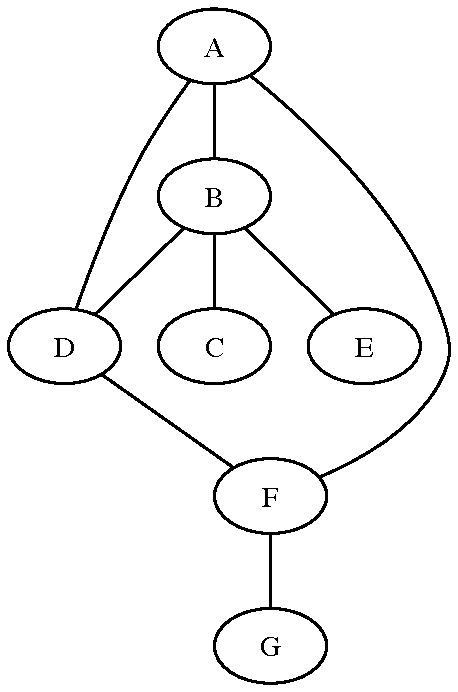
\includegraphics[width=0.2\textwidth]{example-graph}
\end{figure}

Git 提交图相比一般图有一些额外的特性：
\begin{itemize}
    \item 它的边有方向：从子节点指向父节点。我们通常用小的箭头来表示。这样的图被称为有向图。
    \item 它没有循环或``环路"：在上面的例子中，A、D 和 F 之间存在一个循环：你可以在这三个节点之间永远``走"下去。在 Git 历史中，你可以从任意提交开始，走到它的父提交，然后重复：你永远不会遇到循环，而总是会到达一个没有父提交的根提交。Git 历史是无环的。
\end{itemize}
一个既有向又无环的图，猜猜叫什么？有向无环图。这个名字有点拗口，通常简称为 DAG。Git 历史就是一个 DAG。下面是一个简化的历史示例。注意，虽然时间从下往上流动（最近的提交在顶部），但箭头从上往下指向每个提交的祖先。这是因为，正如我们之前看到的，提交指向它们的父提交，而不是子提交。
\begin{figure}[H]
\centering
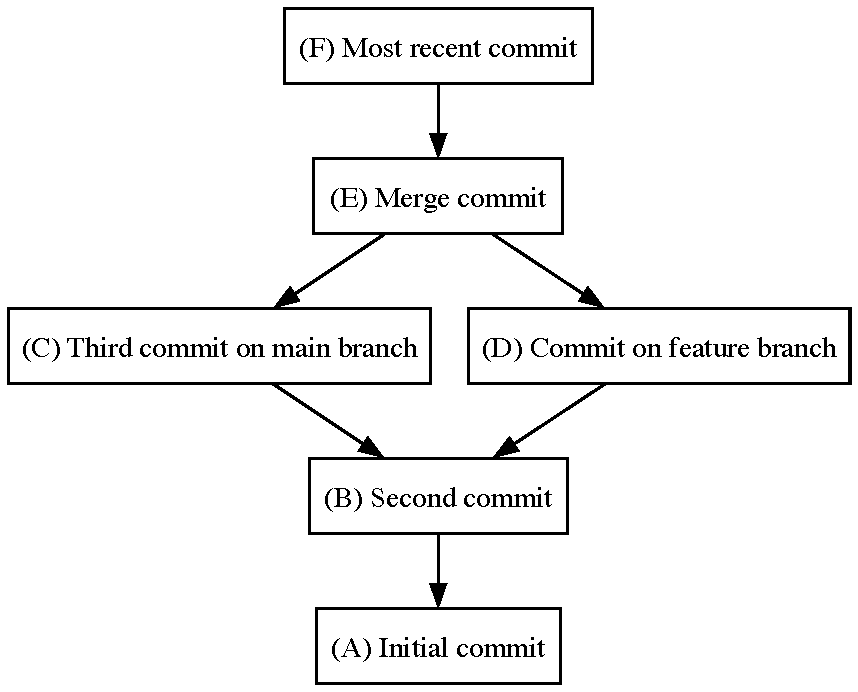
\includegraphics[width=0.55\textwidth]{example-history}
\end{figure}

注意合并提交 E，它有两个祖先。两个分支 C 和 D（可能是一个主分支和一个特性分支）都从一个共同的祖先 B（主分支的较早状态）分叉出来，然后在 E 中合并。由此产生的图形形状就是为什么三点合并（共同祖先加两个变体）有时也被称为 diamond merge（菱形合并）。

\subsubsection{从 DAG 到 Merkle DAG}
所以 Git 提交历史是一个有向无环图（DAG）。它的节点是提交，边是每个提交存储的对父提交的引用。这个历史还有另一个显著特征：与常规图不同，节点的父节点是该节点身份的一部分。这是因为在 Git 中，真正的提交/节点不像上面的例子那样被称为 A、B、C……它们的名字，就像 Git 存储的任何对象的名字一样，是其内容的加密哈希值；而这些内容包括父提交的名字。这意味着一个提交的名字与其在整个历史中的位置绑定，一直到第一个提交。

这是我们在前面已经看到过的：对象的名字不是我们任意决定的，而是对对象应用 SHA-1 函数的结果，这会产生像 \lstinline|6db691fb5486e8f9653e3a63880c9b23885bdfd8| 这样的名字。因此，这些名字在某种意义上不是我们决定的，而是我们发现的。

节点（提交）根据其内容被标记这一事实，使得 Git 历史成为一种类似于 Merkle 树的结构。Merkle 树是一种图，其中每个节点由其内容和子节点内容（一直到终端叶节点）的加密哈希值来标识。这意味着树根的标签同时对树的结构和该结构中每个节点的内容进行了哈希。换句话说，如果你向 Merkle 树追加任何内容，你会修改其所有祖先的身份。

Git 实际使用的数据结构在两个方面与经典的 Merkle 树不同。

首先，它实际上不是一棵树。在计算机科学中，树是一种节点最多有一个祖先的 DAG。在 Git 中，合并提交有多个祖先（它所合并的提交），就像上面例子中的提交 E。（你仍然可能在讨论 Git 历史时看到``Merkle 树"这个名字，但从技术上讲这是不正确的）。

第二个区别在于，在 Git 中，哈希操作是从叶子向根方向进行的。在常规的 Merkle 树中，添加一个额外的提交会改变根的身份，因为根对其叶子进行哈希。但那将意味着添加一个新提交会改变整个历史。Git 所做的恰恰相反：你可以自由地向现有历史追加新提交而不改变它，但每个新提交都与其之前的所有历史绑定。

要理解这是如何工作的，让我们再看看提交对象。这是由 wyag 测试脚本生成的一个提交：
\begin{lstlisting}[language=bash]
tree 8a617fb80c95a1bb638911ae1162ead88282c0eb
parent b664cefa3649658a1dad03163d22cc37ddcd3b77
author wyag-tests.sh <wyag@example.com> 1262304123 +0100
committer wyag-tests.sh <wyag@example.com> 1262304123 +0100

Commit 2
\end{lstlisting}
正如我们之前看到的，这个对象的身份（它的哈希值）是通过对其进行哈希（加上一些额外的头部）计算出来的，得到一个 SHA-1 十六进制哈希值，在这个例子中是 \lstinline|75ee472e7e7021b1639507e89da14b89bfa8987f|。这意味着我们不能给它一个不同的父提交，或者改变它的树，或者改变该提交的任何其他属性而不改变这个哈希 ID。

要创建一个以此提交为父提交的新提交，新提交只需要有一个相应的 parent 字段：
\begin{lstlisting}[language=bash]
...
parent 75ee472e7e7021b1639507e89da14b89bfa8987f
...
\end{lstlisting}
这就是与常规 Merkle 树的关键区别。Git 节点（提交）存储对父提交的引用，而不是对子提交的引用。在现有提交之上添加提交对其祖先没有影响。

这种数据结构的一个基本属性是：你不能修改或移动一个节点而不改变其名字。更戏剧化地说，这意味着节点是不可变的——你根本不能改变或移动它们。你可能认为是修改提交的操作（如 --amend 或 rebase）实际上创建了一个新的提交对象，并保留旧对象供以后进行垃圾回收。

这就是为什么对早期状态的任何修改都会影响所有后续状态。在上面 Git 历史的示例图中，假设我不小心在提交 B 中提交了一个秘密密码。如果我试图``修改" B，我将创建一个新的提交 $B'$，其树稍有不同（没有泄露的密码）。因为树不同了，$B'$ 将有一个不同于 B 的哈希值。为了让 $B'$``成为"C 和 D 的父提交，我需要将 C 和 D 复制为 $C'$ 和 $D'$，修改它们的父字段以匹配 $B'$ 的哈希值。同样的操作将重复进行，在 $C'$ 和 $D'$ 的子节点创建 $E'$，依此类推。这就是重写后历史的样子：
\begin{figure}[H]
\centering
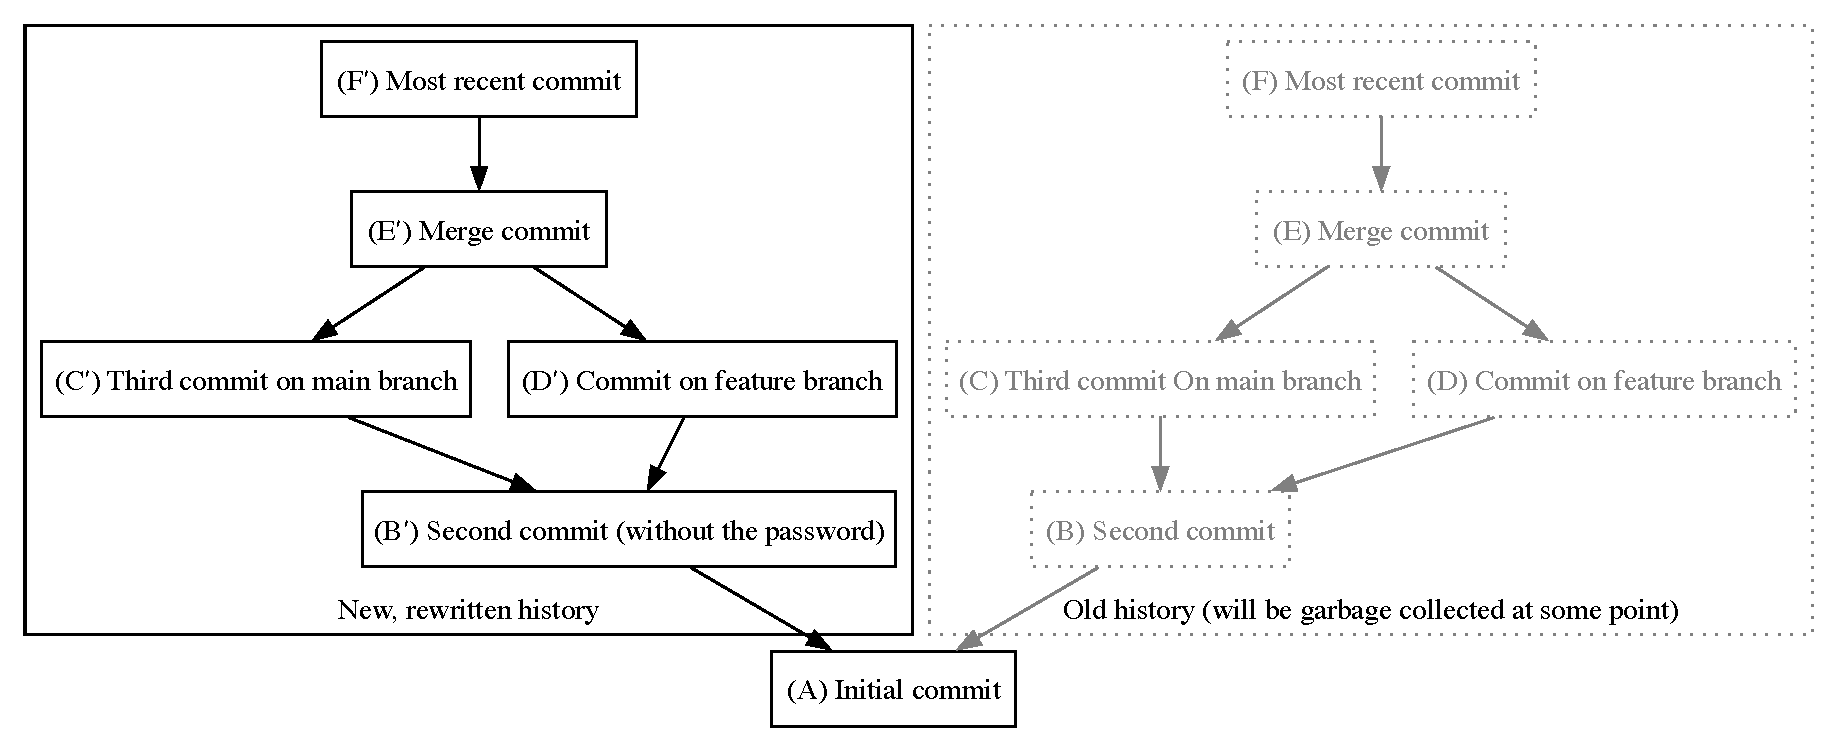
\includegraphics[width=1\textwidth]{example-history-rewrite}
\end{figure}

顺便说一句，这也意味着 Git 历史本质上是无环的：由于对象的身份（其哈希值）递归地依赖于其每个父节点直到根节点的身份，循环将意味着这个递归永远不会终止。更实际地说，试图用两个互相引用对方为父节点的对象创建一个循环，需要在计算另一个对象的哈希值之前知道该对象的哈希值。

    \begin{remark}等等，这看起来像……区块链？

    Merkle 树的一个非常常见的用途是在所谓的``加密货币"的区块链中。例如在比特币中，账本就是一个 Merkle 树。``挖矿"包括向链中添加新交易（这是容易的部分），然后找到一种方法用使最终哈希值以给定数量的二进制 1 开头的值来填充区块（这就是``工作量证明"，故意使网络变慢且耗能，以防止其分叉）。

    所以是的，在某种意义上，Git 是一个区块链：它是由加密手段连接在一起的区块（提交）序列，确保每个元素都与整个历史结构相关联。不过不要太当真：我们不需要 GitCoin。真的，不需要。
    \end{remark}

\section{读取提交数据：checkout}
让我们继续处理提交对象。知道它们在一个给定的状态中包含的远不止文件和目录固然很好，但这并不能让它们真正有用。现在可能是时候开始实现树（tree）对象了，这样我们就能够将提交检出（checkout）到工作树中。
\subsection{树中包含什么？}
非正式地说，树描述了工作树的内容，即它将 blob 与路径关联起来。它是由文件模式、路径（相对于工作树）和 SHA-1 组成的三元组数组。一个典型的树内容可能如下所示：
\begin{table}[H]
\centering
\begin{tabular}{l l l}
\toprule
\textbf{Mode} & \textbf{SHA-1} & \textbf{Path} \\
\midrule
\lstinline|100644| & \lstinline|894a44cc066a027465cd26d634948d56d13af9af| & \lstinline|.gitignore| \\
\lstinline|100644| & \lstinline|94a9ed024d3859793618152ea559a168bbcbb5e2| & \lstinline|LICENSE| \\
\lstinline|100644| & \lstinline|bab489c4f4600a38ce6dbdf652b90383a4aa3e45| & \lstinline|README.md| \\
\lstinline|100644| & \lstinline|6d208e47659a2a10f5f8640e0155d9276a2130a9| & \lstinline|src| \\
\lstinline|040000| & \lstinline|e7445b03aea61ec801b20d6ab62f076208b7d097| & \lstinline|tests| \\
\lstinline|040000| & \lstinline|d5ec863f17f3a2e92aa8f6b66ac18f7b09fd1b38| & \lstinline|main.c| \\
\bottomrule
\end{tabular}
\end{table}
模式就是文件的模式，路径是它的位置。SHA-1 引用的是 blob 对象或另一个树对象。如果是 blob，则路径是文件；如果是树，则路径是目录。要在文件系统中实例化这棵树，我们将从加载与第一个路径（.gitignore）关联的对象并检查其类型开始。由于它是一个 blob，我们只需创建一个名为 .gitignore 的文件，内容为该 blob 的内容；LICENSE 和 README.md 同理。但与 src 关联的对象不是 blob，而是另一个树：我们将创建 src 目录，并在该目录中使用新的树重复相同的操作。
\begin{warning}
    一个路径对应一个文件系统条目

    路径精确地标识一个文件或目录。不是两个，也不是三个。如果你有五层嵌套目录，即使除了下一层目录外有四层是空的，你也需要五个递归引用彼此的树对象。你不能走捷径将完整路径放在单个树条目中，比如 \lstinline|dir1/dir2/dir3/dir4/dir5|。\end{warning}

\subsection{解析树对象}
与标签和提交不同，树对象是二进制对象，但它们的格式实际上相当简单。一棵树是以下格式记录的连接：
\begin{lstlisting}[language=bash]
[mode] space [path] 0x00 [sha-1]
\end{lstlisting}
\begin{itemize}
    \item \lstinline|[mode]| 最多 6 个字节，是文件模式的八进制表示，以 ASCII 存储。例如，100644 编码为字节值 49（ASCII ``1"）、48（ASCII ``0"）、48、54、52、52。前两位编码文件类型（文件、目录、符号链接或子模块），后四位是其权限。
    \item 后面跟着 0x20，一个 ASCII 空格；
    \item 后面跟着以空字节（0x00）结尾的路径；
    \item 后面跟着对象的 SHA-1，以二进制编码，占 20 个字节。
\end{itemize}
解析器将非常简单。首先，为单个记录（一个叶子，一个路径）创建一个小的对象包装器：
\begin{lstlisting}[language=Python]
class GitTreeLeaf (object):
    def __init__(self, mode, path, sha):
        self.mode = mode
        self.path = path
        self.sha = sha
\end{lstlisting}
因为树对象只是相同基本数据结构的重复，我们将解析器写成两个函数。首先是一个提取单个记录的解析器，返回解析后的数据以及它在输入数据中达到的位置：
\begin{lstlisting}[language=Python]
def tree_parse_one(raw, start=0):
    # Find the space terminator of the mode
    x = raw.find(b' ', start)
    assert x-start == 5 or x-start==6

    # Read the mode
    mode = raw[start:x]
    if len(mode) == 5:
        # Normalize to six bytes.
        mode = b"0" + mode

    # Find the NULL terminator of the path
    y = raw.find(b'\x00', x)
    # and read the path
    path = raw[x+1:y]

    # Read the SHA…
    raw_sha = int.from_bytes(raw[y+1:y+21], "big")
    # and convert it into an hex string, padded to 40 chars
    # with zeros if needed.
    sha = format(raw_sha, "040x")
    return y+21, GitTreeLeaf(mode, path.decode("utf8"), sha)
\end{lstlisting}
而``真正的"解析器只是在循环中调用上述函数，直到输入数据耗尽：
\begin{lstlisting}[language=Python]
def tree_parse(raw):
    pos = 0
    max = len(raw)
    ret = list()
    while pos < max:
        pos, data = tree_parse_one(raw, pos)
        ret.append(data)

    return ret
\end{lstlisting}

\subsection{写入树对象}
我们最终需要一个序列化器来写回树对象。因为我们可能添加或修改了条目，所以需要再次对它们进行排序。一致的排序很重要，因为我们需要尊重 Git 的身份规则，该规则规定两个等价的对象不能有不同的哈希值——但具有相同内容但排序不同的树将是等价的（描述相同的目录结构），然而数值上却是不同的（不同的 SHA-1 标识符）。排序不正确的树是无效的，但 Git 并不强制执行这一点。我在编写 wyag 时曾意外创建过一些无效的树，结果在 git status 中遇到了奇怪的 bug（具体来说，status 会将一个实际上干净的工作树报告为完全修改）。我们不希望这样。

排序函数相当简单，但有一个小变化。条目按名称字母顺序排序，但目录名称（即树条目）在右侧用单个斜杠 / 填充。如果 foo 是一个普通文件，它会在 foo.c 之前排序；但如果 foo 是一个目录，它会在 foo.c 之后排序（因为 foo/）。这个额外规则的结果（以及可能的原因）是 \lstinline|git ls-tree -r| 可以简单地遍历对象并按字典顺序输出路径列表：
\begin{lstlisting}[language=bash]
$ git ls-tree -r HEAD
foo.c
foo/bar.c
\end{lstlisting}
这种填充仅在排序时考虑：最终的 / 永远不会出现在树对象本身中。这个小函数为目录名称添加最后的 / 以用于排序：
\begin{lstlisting}[language=Python]
# Notice this isn't a comparison function, but a conversion function.
# Python's default sort doesn't accept a custom comparison function,
# like in most languages, but a `key` arguments that returns a new
# value, which is compared using the default rules.  So we just return
# the leaf name, with an extra / if it's a directory.
def tree_leaf_sort_key(leaf):
    if leaf.mode.startswith(b"4"):
        return leaf.path + "/"
    else:
        return leaf.path
\end{lstlisting}
然后是序列化器本身。这非常简单：我们使用新创建的函数作为转换器对项目进行排序，然后按顺序写入它们。
\begin{lstlisting}[language=Python]
def tree_serialize(obj):
    obj.items.sort(key=tree_leaf_sort_key)
    ret = b''
    for i in obj.items:
        ret += i.mode
        ret += b' '
        ret += i.path.encode("utf8")
        ret += b'\x00'
        sha = int(i.sha, 16)
        ret += sha.to_bytes(20, byteorder="big")
    return ret
\end{lstlisting}
现在我们只需将所有这些组合成一个类：
\begin{lstlisting}[language=Python]
class GitTree(GitObject):
    fmt=b'tree'

    def deserialize(self, data):
        self.items = tree_parse(data)

    def serialize(self):
        return tree_serialize(self)

    def init(self):
        self.items = list()
\end{lstlisting}
\cprotect\subsection{显示树对象：\verb|ls-tree|}
趁热打铁，让我们为 wyag 添加 ls-tree 命令。这非常简单，没有理由不实现。\lstinline|git ls-tree [-r] TREE| 的作用是打印树的内容，使用 -r 标志时可以递归打印。在递归模式下，它不显示子树，只显示带有完整路径的最终对象。
\begin{lstlisting}[language=Python]
argsp = argsubparsers.add_parser("ls-tree", help="Pretty-print a tree object.")
argsp.add_argument("-r",
                   dest="recursive",
                   action="store_true",
                   help="Recurse into sub-trees")

argsp.add_argument("tree",
                   help="A tree-ish object.")

def cmd_ls_tree(args):
    repo = repo_find()
    ls_tree(repo, args.tree, args.recursive)

def ls_tree(repo, ref, recursive=None, prefix=""):
    sha = object_find(repo, ref, fmt=b"tree")
    obj = object_read(repo, sha)
    for item in obj.items:
        if len(item.mode) == 5:
            type = item.mode[0:1]
        else:
            type = item.mode[0:2]

        match type: # Determine the type.
            case b'04': type = "tree"
            case b'10': type = "blob" # A regular file.
            case b'12': type = "blob" # A symlink. Blob contents is link target.
            case b'16': type = "commit" # A submodule
            case _: raise Exception(f"Weird tree leaf mode {item.mode}")

        if not (recursive and type=='tree'): # This is a leaf
            print(f"{'0' * (6 - len(item.mode)) + item.mode.decode('ascii')} {type} {item.sha}\t{os.path.join(prefix, item.path)}")
        else: # This is a branch, recurse
            ls_tree(repo, item.sha, recursive, os.path.join(prefix, item.path))
\end{lstlisting}
运行结果类似如下：
\begin{lstlisting}[language=bash]
$ ./wyag ls-tree HEAD
100644 blob 0e03663b6cefce83bea24d48d9c887c4bc011025    .gitignore
100644 blob 9cb35991783976a6c5fc51013f429940f63e08fb    .gitmodules
100644 blob 94a9ed024d3859793618152ea559a168bbcbb5e2    LICENSE
100644 blob 25846e47b3da80a34190b4d60c149589428b4957    Makefile
100644 blob e0695f14a412c29e252c998c81de1dde59658e4a    README.org
040000 tree 7e8315f7ba77e713da38e84d8af3ffc5b80b6e00    lib
100644 blob aafc00f9f92091f141982363e0a16f612819e19f    write-yourself-a-git.org
100755 blob ec673d798f6a5a4273a89543d6a667be3836bd37    wyag-tests.sh
\end{lstlisting}
\cprotect\subsection{\verb|checkout| 命令}
git checkout 的作用是在工作树中实例化一个提交。为了保持我们的实现清晰易懂，我们将对实际的 git 命令进行极大的简化。我们还将添加一些安全保护措施。以下是我们的 checkout 版本的工作方式：
\begin{itemize}
    \item 它接受两个参数：一个提交和一个目录。而 Git checkout 只需要一个提交。
    \item 然后，当且仅当目录为空时，它才会在该目录中实例化树。Git 充满了避免删除数据的安全保护措施，要在 wyag 中尝试复现这些措施会过于复杂且不安全。由于 wyag 的目的是演示 Git 的工作原理，而不是产生一个可用的实现，这个限制是可以接受的。
\end{itemize}
让我们开始吧。像往常一样，我们需要一个子解析器：
\begin{lstlisting}[language=Python]
argsp = argsubparsers.add_parser("checkout", help="Checkout a commit inside of a directory.")

argsp.add_argument("commit",
                   help="The commit or tree to checkout.")

argsp.add_argument("path",
                   help="The EMPTY directory to checkout on.")
\end{lstlisting}
包装函数：
\begin{lstlisting}[language=Python]
def cmd_checkout(args):
    repo = repo_find()

    obj = object_read(repo, object_find(repo, args.commit))

    # If the object is a commit, we grab its tree
    if obj.fmt == b'commit':
        obj = object_read(repo, obj.kvlm[b'tree'].decode("ascii"))

    # Verify that path is an empty directory
    if os.path.exists(args.path):
        if not os.path.isdir(args.path):
            raise Exception(f"Not a directory {args.path}!")
        if os.listdir(args.path):
            raise Exception(f"Not empty {args.path}!")
    else:
        os.makedirs(args.path)

    tree_checkout(repo, obj, os.path.realpath(args.path))
\end{lstlisting}
以及执行实际工作的函数：
\begin{lstlisting}[language=Python]
def tree_checkout(repo, tree, path):
    for item in tree.items:
        obj = object_read(repo, item.sha)
        dest = os.path.join(path, item.path)

        if obj.fmt == b'tree':
            os.mkdir(dest)
            tree_checkout(repo, obj, dest)
        elif obj.fmt == b'blob':
            # @TODO Support symlinks (identified by mode 12****)
            with open(dest, 'wb') as f:
                f.write(obj.blobdata)
\end{lstlisting}
\section{引用、标签和分支}
\cprotect\subsection{什么是引用，以及 \verb|show-ref| 命令}
到目前为止，我们引用对象的唯一方式是使用它们的完整十六进制标识符。在 Git 中，我们实际上很少看到这些，除非是在谈论特定的提交。但在一般情况下，我们谈论的是 HEAD，或者像 \lstinline|main| 或 \lstinline|feature/more-bombs| 这样的分支名称，等等。这些由一个称为引用的简单机制来处理。

Git 引用（refs）可能是 Git 保存的最简单的数据类型。它们位于 \lstinline|.git/refs| 的子目录中，是包含对象哈希的十六进制表示（以 ASCII 编码）的文本文件。它们实际上就这么简单：
\begin{lstlisting}[language=bash]
6071c08bcb4757d8c89a30d9755d2466cef8c1de
\end{lstlisting}
引用也可以引用另一个引用，从而间接地指向一个对象，这时它们看起来像这样：
\begin{lstlisting}[language=bash]
ref: refs/remotes/origin/master
\end{lstlisting}
\begin{remark}
直接引用和间接引用

从现在开始，我将把形式为 \lstinline|ref: path/to/other/ref| 的引用称为间接引用，把包含 SHA-1 对象 ID 的引用称为直接引用。
\end{remark}
本节将描述引用的用途。目前，重要的只有以下几点：
\begin{itemize}
    \item 它们是文本文件，位于 \lstinline|.git/refs| 层级结构中；
    \item 它们保存对象的 SHA-1 标识符，或对另一个引用的引用（最终指向一个 SHA-1，没有循环！）。
\end{itemize}
为了处理引用，我们首先需要一个简单的递归解析器，它接受一个引用名称，跟随可能的递归引用（内容以 ref: 开头的引用，如上例所示），并返回一个 SHA-1 标识符：
\begin{lstlisting}[language=Python]
def ref_resolve(repo, ref):
    path = repo_file(repo, ref)

    # Sometimes, an indirect reference may be broken.  This is normal
    # in one specific case: we're looking for HEAD on a new repository
    # with no commits.  In that case, .git/HEAD points to "ref:
    # refs/heads/main", but .git/refs/heads/main doesn't exist yet
    # (since there's no commit for it to refer to).
    if not os.path.isfile(path):
        return None

    with open(path, 'r') as fp:
        data = fp.read()[:-1]
        # Drop final \n ^^^^^
    if data.startswith("ref: "):
        return ref_resolve(repo, data[5:])
    else:
        return data
\end{lstlisting}
让我们创建两个小函数，并实现 show-ref 命令——它只是列出仓库中的所有引用。首先，一个简单的递归函数来收集引用并将它们作为字典返回：
\begin{lstlisting}[language=Python]
def ref_list(repo, path=None):
    if not path:
        path = repo_dir(repo, "refs")
    ret = dict()
    # Git shows refs sorted.  To do the same, we sort the output of
    # listdir
    for f in sorted(os.listdir(path)):
        can = os.path.join(path, f)
        if os.path.isdir(can):
            ret[f] = ref_list(repo, can)
        else:
            ret[f] = ref_resolve(repo, can)

    return ret
\end{lstlisting}
然后，像往常一样，一个子解析器、一个桥接函数和一个（递归的）工作函数：
\begin{lstlisting}[language=Python]
argsp = argsubparsers.add_parser("show-ref", help="List references.")

def cmd_show_ref(args):
    repo = repo_find()
    refs = ref_list(repo)
    show_ref(repo, refs, prefix="refs")

def show_ref(repo, refs, with_hash=True, prefix=""):
    if prefix:
        prefix = prefix + '/'
    for k, v in refs.items():
        if type(v) == str and with_hash:
            print (f"{v} {prefix}{k}")
        elif type(v) == str:
            print (f"{prefix}{k}")
        else:
            show_ref(repo, v, with_hash=with_hash, prefix=f"{prefix}{k}")
\end{lstlisting}
\subsection{标签作为引用}
引用最简单的用途是标签。标签只是用户为对象（通常是提交）定义的名称。标签的一个非常常见的用途是标识软件版本：假设你刚刚合并了程序版本 \lstinline|12.78.52| 的最后一个提交，那么你最近的提交（我们称它为 \lstinline|6071c08|）就是你的版本 \lstinline|12.78.52|。要显式地建立这个关联，你只需执行：
\begin{lstlisting}[language=bash]
git tag v12.78.52 6071c08
# the object hash ^here^^ is optional and defaults to HEAD.
\end{lstlisting}
这会创建一个名为 \lstinline|v12.78.52| 的新标签，指向 \lstinline|6071c08|。标签类似于别名：它引入了一种引用现有对象的新方式。标签创建后，名称 \lstinline|v12.78.52| 就指向了 \lstinline|6071c08|。例如，以下两个命令现在完全等价：
\begin{lstlisting}[language=bash]
git checkout v12.78.52
git checkout 6071c08
\end{lstlisting}
\begin{remark}
版本是标签的常见用途，但像 Git 中的几乎所有东西一样，标签没有预定义的语义：它们意味着你想要的任何含义，可以指向任何你想要的对象，你甚至可以给 blob 打标签！
\end{remark}
\subsection{轻量级标签和标签对象，以及后者的解析}
你可能已经猜到，标签实际上就是引用。它们位于 \lstinline|.git/refs/tags/| 层级结构中。唯一值得注意的一点是，它们有两种形式：轻量级标签和标签对象。
\begin{description}
    \item[``轻量级"标签] 只是指向提交、树或 blob 的普通引用。
    \item[标签对象] 是指向 tag 类型对象的普通引用。与轻量级标签不同，标签对象有作者、日期、可选的 PGP 签名和可选的附注。它们的格式与提交对象相同。
\end{description}
我们甚至不需要实现标签对象，可以直接复用 GitCommit，只需更改 fmt 字段：
\begin{lstlisting}[language=Python]
class GitTag(GitCommit):
    fmt = b'tag'
\end{lstlisting}
现在我们就支持标签了。
\cprotect\subsection{\verb|tag| 命令}
让我们添加 tag 命令。在 Git 中，它做两件事：创建新标签或列出已有标签（默认行为）。因此，你可以这样调用：
\begin{lstlisting}[language=bash]
git tag                  # List all tags
git tag NAME [OBJECT]    # create a new *lightweight* tag NAME, pointing
                         # at HEAD (default) or OBJECT
git tag -a NAME [OBJECT] # create a new tag *object* NAME, pointing at
                         # HEAD (default) or OBJECT
\end{lstlisting}
这可以转换为如下的 argparse 代码。注意我们忽略了 \lstinline|--list| 和 \lstinline|[-a] name [object]| 之间的互斥关系，这对 argparse 来说似乎太复杂了。
\begin{lstlisting}[language=Python]
argsp = argsubparsers.add_parser(
    "tag",
    help="List and create tags")

argsp.add_argument("-a",
                   action="store_true",
                   dest="create_tag_object",
                   help="Whether to create a tag object")

argsp.add_argument("name",
                   nargs="?",
                   help="The new tag's name")

argsp.add_argument("object",
                   default="HEAD",
                   nargs="?",
                   help="The object the new tag will point to")
\end{lstlisting}
\lstinline|cmd_tag| 函数将根据是否提供了 name 来分派行为（列出或创建）：
\begin{lstlisting}[language=Python]
def cmd_tag(args):
    repo = repo_find()

    if args.name:
        tag_create(repo,
                   args.name,
                   args.object,
                   create_tag_object = args.create_tag_object)
    else:
        refs = ref_list(repo)
        show_ref(repo, refs["tags"], with_hash=False)
\end{lstlisting}
我们只需要再一个函数来实际创建标签：
\begin{lstlisting}[language=Python]
def tag_create(repo, name, ref, create_tag_object=False):
    # get the GitObject from the object reference
    sha = object_find(repo, ref)

    if create_tag_object:
        # create tag object (commit)
        tag = GitTag()
        tag.kvlm = dict()
        tag.kvlm[b'object'] = sha.encode()
        tag.kvlm[b'type'] = b'commit'
        tag.kvlm[b'tag'] = name.encode()
        # Feel free to let the user give their name!
        # Notice you can fix this after commit, read on!
        tag.kvlm[b'tagger'] = b'Wyag <wyag@example.com>'
        # …and a tag message!
        tag.kvlm[None] = b"A tag generated by wyag, which won't let you customize the message!\n"
        tag_sha = object_write(tag, repo)
        # create reference
        ref_create(repo, "tags/" + name, tag_sha)
    else:
        # create lightweight tag (ref)
        ref_create(repo, "tags/" + name, sha)

def ref_create(repo, ref_name, sha):
    with open(repo_file(repo, "refs/" + ref_name), 'w') as fp:
        fp.write(sha + "\n")
\end{lstlisting}
\subsection{什么是分支？}
标签完成了。现在是另一个大块：分支。

是时候解决房间里的大象了：像大多数 Git 用户一样，wyag 仍然不知道分支是什么。它目前将仓库视为一堆无序的对象，其中一些是提交，完全没有表示提交被分组到分支中的事实，以及在每个时间点都有一个提交是 HEAD，即活动分支的头提交（或``tip"）。

那么，什么是分支？答案实际上出奇地简单，但也可能只是让人惊讶：分支是指向提交的引用。你甚至可以说分支是提交的一种名称。在这方面，分支与标签完全相同。标签是位于 \lstinline|.git/refs/tags| 中的引用，分支是位于 \lstinline|.git/refs/heads| 中的引用。

当然，分支和标签之间有一些区别：
\begin{enumerate}
    \item 标签可以指向任何对象，而分支是指向提交的引用；
    \item 最重要的是，分支引用在每次提交时都会更新。这意味着每当你提交时，Git 实际上会执行以下操作：
    \begin{enumerate}[label=\arabic*.]
        \item 创建一个新的提交对象，以当前分支的 ID（提交的 ID！）作为其父提交；
        \item 提交对象被哈希并存储；
        \item 分支引用被更新以指向新提交的哈希值。
    \end{enumerate}
\end{enumerate}
就是这样。

那么当前分支呢？实际上更简单。它是一个位于 refs 层级之外的引用文件，在 \lstinline|.git/HEAD| 中，它是一个间接引用（即它的形式是 \lstinline|ref: path/to/other/ref|，而不是一个简单的哈希）。

    \begin{remark}分离的 HEAD

    当你只是检出一个随机的提交时，Git 会警告你处于``分离的 HEAD 状态"。这意味着你不再在任何分支上。在这种情况下，\lstinline|.git/HEAD| 是一个直接引用：它包含一个 SHA-1。\end{remark}

\cprotect\subsection{引用对象：\verb|object_find| 函数}
\subsubsection{名称解析}
还记得我们之前创建的那个愚蠢的 \verb|object_find| 函数吗？它接受四个参数，原封不动地返回第二个参数而忽略其他三个。现在是时候用一个更有用的版本来替换它了。我们将实现实际 Git 名称解析算法的一个小子集，但已经足够使用。新的 \verb|object_find()| 将分两步工作：首先，给定一个名称，它返回一个完整的 SHA-1 哈希值。例如，对于 HEAD，它将返回当前分支头提交的哈希值。更精确地说，这个名称解析函数将这样工作：
\begin{itemize}
    \item 如果名称是 HEAD，就解析 \lstinline|.git/HEAD|；
    \item 如果名称是完整的哈希值，则原样返回该哈希值；
    \item 如果名称看起来像短哈希，则收集所有完整哈希以此短哈希开头的对象；
    \item 最后，解析与名称匹配的标签和分支。
\end{itemize}
注意后两步是如何收集值的：前两步是绝对引用，所以我们可以安全地返回结果。但短哈希或分支名称可能有歧义，我们需要枚举名称的所有可能含义，如果找到多于一个则抛出错误。

短哈希：为了方便，Git 允许使用哈希值的前缀来引用它。例如，\lstinline|5bd254aa973646fa16f66d702a5826ea14a3eb45| 可以被引用为 \lstinline|5bd254|。这被称为``短哈希"。
\begin{lstlisting}[language=Python]
def object_resolve(repo, name):
    """Resolve name to an object hash in repo.

This function is aware of:

 - the HEAD literal
    - short and long hashes
    - tags
    - branches
    - remote branches"""
    candidates = list()
    hashRE = re.compile(r"^[0-9A-Fa-f]{4,40}$")

    # Empty string?  Abort.
    if not name.strip():
        return None

    # Head is nonambiguous
    if name == "HEAD":
        return [ ref_resolve(repo, "HEAD") ]

    # If it's a hex string, try for a hash.
    if hashRE.match(name):
        # This may be a hash, either small or full.  4 seems to be the
        # minimal length for git to consider something a short hash.
        # This limit is documented in man git-rev-parse
        name = name.lower()
        prefix = name[0:2]
        path = repo_dir(repo, "objects", prefix, mkdir=False)
        if path:
            rem = name[2:]
            for f in os.listdir(path):
                if f.startswith(rem):
                    # Notice a string startswith() itself, so this
                    # works for full hashes.
                    candidates.append(prefix + f)

    # Try for references.
    as_tag = ref_resolve(repo, "refs/tags/" + name)
    if as_tag: # Did we find a tag?
        candidates.append(as_tag)

    as_branch = ref_resolve(repo, "refs/heads/" + name)
    if as_branch: # Did we find a branch?
        candidates.append(as_branch)

    as_remote_branch = ref_resolve(repo, "refs/remotes/" + name)
    if as_remote_branch: # Did we find a remote branch?
        candidates.append(as_remote_branch)

    return candidates
\end{lstlisting}
第二步，如果提供了类型参数，则跟踪找到的对象直到所需类型。由于我们只需要处理简单的情况，这是一个非常简单的迭代过程：
\begin{itemize}
    \item 如果找到的是标签而 fmt 是其他类型，则跟踪标签；
    \item 如果找到的是提交而 fmt 是 tree，则返回该提交的树对象；
    \item 在其他所有情况下，退出：没有其他合理的解释。
\end{itemize}
（这个过程是迭代的，因为可能需要不确定的步数，因为标签本身也可以被标记）
\begin{lstlisting}[language=Python]
def object_find(repo, name, fmt=None, follow=True):
    sha = object_resolve(repo, name)

    if not sha:
        raise Exception(f"No such reference {name}.")

    if len(sha) > 1:
        raise Exception(f"Ambiguous reference {name}: Candidates are:\n - {'\n - '.join(sha)}.")

    sha = sha[0]

    if not fmt:
        return sha

    while True:
        obj = object_read(repo, sha)
        #     ^^^^^^^^^^^ < this is a bit agressive: we're reading
        # the full object just to get its type.  And we're doing
        # that in a loop, albeit normally short.  Don't expect
        # high performance here.

        if obj.fmt == fmt:
            return sha

        if not follow:
            return None

        # Follow tags
        if obj.fmt == b'tag':
            sha = obj.kvlm[b'object'].decode("ascii")
        elif obj.fmt == b'commit' and fmt == b'tree':
            sha = obj.kvlm[b'tree'].decode("ascii")
        else:
            return None
\end{lstlisting}
有了新的 \lstinline|object_find()|，CLI 版本的 wyag 变得更可用了。现在你可以做这样的事情：
\begin{lstlisting}[language=bash]
$ wyag checkout v3.11 tmp/ # A tag
$ wyag checkout feature/explosions tmp/ # A branch
$ wyag ls-tree -r HEAD # The active branch or commit.  There's also a
                       # follow here: HEAD is actually a commit.
$ wyag cat-file blob e0695f # A short hash
$ wyag cat-file tree master # A branch, as a tree (another "follow")
\end{lstlisting}
\subsubsection{rev-parse 命令}
让我们实现 wyag rev-parse。git rev-parse 命令做很多事情，但我们将复制的其中一个用例是解析引用。为了进一步测试 \lstinline|object_find| 的``跟踪"功能，我们将在其接口中添加一个可选的 --wyag-type 参数。
\begin{lstlisting}[language=Python]
argsp = argsubparsers.add_parser(
    "rev-parse",
    help="Parse revision (or other objects) identifiers")

argsp.add_argument("--wyag-type",
                   metavar="type",
                   dest="type",
                   choices=["blob", "commit", "tag", "tree"],
                   default=None,
                   help="Specify the expected type")

argsp.add_argument("name",
                   help="The name to parse")
\end{lstlisting}
桥接函数完成所有工作：
\begin{lstlisting}[language=Python]
def cmd_rev_parse(args):
    if args.type:
        fmt = args.type.encode()
    else:
        fmt = None

    repo = repo_find()

    print (object_find(repo, args.name, fmt, follow=True))
\end{lstlisting}
它能够正常工作：
\begin{lstlisting}[language=bash]
$ wyag rev-parse --wyag-type commit HEAD
6c22393f5e3830d15395fd8d2f8b0cf8eb40dd58
$ wyag rev-parse --wyag-type tree HEAD
11d33fad71dbac72840aff1447e0d080c7484361
$ wyag rev-parse --wyag-type tag HEAD
None
\end{lstlisting}

\section{使用暂存区和索引文件}
\subsection{什么是索引文件？}
这最后一步将把我们带到提交发生的地方（尽管实际创建提交是下一节的内容！）

你可能知道，要在 Git 中提交，首先需要使用 git add 和 git rm 来``暂存"一些更改，然后才提交这些更改。上次提交和下次提交之间的这个中间阶段称为暂存区。

用提交对象或树对象来表示暂存区似乎是自然的，但 Git 实际上使用了一种完全不同的机制，即所谓的索引文件。

在提交之后，索引文件是该提交的一种副本：它保存与对应树相同的路径/blob 关联。但它还保存了关于工作树中文件的额外信息，比如它们的创建/修改时间，这样 git status 通常不需要实际比较文件：它只需检查文件的修改时间是否与索引文件中存储的相同，只有当不同时才执行实际比较。

因此，你可以把索引文件看作一个三向关联列表：不仅将路径与 blob 关联，还将路径与实际的文件系统条目关联。

索引文件的另一个重要特点是，与树不同，它可以表示不一致的状态，比如合并冲突，而树始终是完整、无歧义的表示。

当你提交时，Git 实际做的是将索引文件转换为一个新的树对象。总结如下：
\begin{enumerate}
    \item 当仓库处于``干净"状态时，索引文件包含与 HEAD 提交完全相同的内容，加上关于相应文件系统条目的元数据。例如，它可能包含类似这样的信息：
      \begin{quote}
There’s a file called src/disp.c whose contents are blob 797441c76e59e28794458b39b0f1eff4c85f4fa0. The real src/disp.c file, in the worktree, was created on 2023-07-15 15:28:29.168572151, and last modified 2023-07-15 15:28:29.1689427709. It is stored on device 65026, inode 8922881.
      \end{quote}
    \item 当你执行 git add 或 git rm 时，索引文件会被相应修改。在上面的例子中，如果你修改了 src/disp.c 并添加了更改，索引文件将更新为新的 blob ID（当然，blob 本身也会在这个过程中被创建），并且各种文件元数据也会被更新，以便 git status 知道何时不需要比较文件内容。
    \item 当你提交这些更改时，会从索引文件生成一个新的树，用该树生成一个新的提交对象，分支被更新，完成操作。
\end{enumerate}
    \begin{remark}关于术语

    暂存区和索引是同一回事，但``暂存区"更像是 Git 面向用户的功能名称（本可以用其他方式实现），是抽象概念；而``索引文件"特指这个抽象功能在 Git 中的实际实现方式。\end{remark}
\subsection{解析索引文件}
索引文件是 Git 仓库能保存的最复杂的数据结构。它的完整文档可以在 Git 源代码树中找到，或者在 Git 网站上查看。它由三部分组成：
\begin{itemize}
    \item 一个头部，包含格式版本号和索引中的条目数量；
    \item 一系列条目，已排序，每个代表一个文件；填充到 8 字节的倍数；
    \item 一系列可选扩展，我们将忽略它们。
\end{itemize}
我们首先需要表示单个条目。它实际上包含相当多的信息，我把细节留在注释中。值得注意的是，一个条目既存储对象存储中关联 blob 的 SHA-1，也存储关于实际文件系统上实际文件的大量元数据。同样，这是因为 \lstinline|git/wyag status| 需要确定索引中的哪些文件被修改了：在实际比较文件之前，首先检查最后修改时间戳并将其与已知值进行比较要高效得多。
\begin{lstlisting}[language=Python]
class GitIndexEntry (object):
    def __init__(self, ctime=None, mtime=None, dev=None, ino=None,
                 mode_type=None, mode_perms=None, uid=None, gid=None,
                 fsize=None, sha=None, flag_assume_valid=None,
                 flag_stage=None, name=None):
        # The last time a file's metadata changed.  This is a pair
        # (timestamp in seconds, nanoseconds)
        self.ctime = ctime
        # The last time a file's data changed.  This is a pair
        # (timestamp in seconds, nanoseconds)
        self.mtime = mtime
        # The ID of device containing this file
        self.dev = dev
        # The file's inode number
        self.ino = ino
        # The object type, either b1000 (regular), b1010 (symlink),
        # b1110 (gitlink).
        self.mode_type = mode_type
        # The object permissions, an integer.
        self.mode_perms = mode_perms
        # User ID of owner
        self.uid = uid
        # Group ID of ownner
        self.gid = gid
        # Size of this object, in bytes
        self.fsize = fsize
        # The object's SHA
        self.sha = sha
        self.flag_assume_valid = flag_assume_valid
        self.flag_stage = flag_stage
        # Name of the object (full path this time!)
        self.name = name
\end{lstlisting}
索引文件是一个二进制文件，可能是出于性能原因。不过格式相当简单。它以包含 DIRC 魔数、版本号和索引文件中条目总数的头部开始。我们创建 GitIndex 类来保存它们：
\begin{lstlisting}[language=Python]
class GitIndex (object):
    version = None
    entries = []
    # ext = None
    # sha = None

    def __init__(self, version=2, entries=None):
        if not entries:
            entries = list()

        self.version = version
        self.entries = entries
\end{lstlisting}
以及一个解析器，用于将索引文件读入这些对象。在读取 12 字节的头部后，我们按条目出现的顺序解析它们。一个条目以一组固定长度的数据开始，后跟一个可变长度的名称。

代码相当直接，但由于它在读取二进制格式，感觉比我们之前做的更混乱。我们大量使用 \lstinline|int.from_bytes(bytes, endianness)| 将原始字节读入整数，并使用少量位运算来分离共享同一字节的数据。

（这种格式可能是这样设计的：索引文件可以直接 mmap() 到内存，并作为 C 结构体直接读取，在大多数情况下以 O(n) 时间构建索引。这种方法在 C 中产生的代码比在 Python 中更优雅……）
\begin{lstlisting}[language=Python]
def index_read(repo):
    index_file = repo_file(repo, "index")

    # New repositories have no index!
    if not os.path.exists(index_file):
        return GitIndex()

    with open(index_file, 'rb') as f:
        raw = f.read()

    header = raw[:12]
    signature = header[:4]
    assert signature == b"DIRC" # Stands for "DirCache"
    version = int.from_bytes(header[4:8], "big")
    assert version == 2, "wyag only supports index file version 2"
    count = int.from_bytes(header[8:12], "big")

    entries = list()

    content = raw[12:]
    idx = 0
    for i in range(0, count):
        # Read creation time, as a unix timestamp (seconds since
        # 1970-01-01 00:00:00, the "epoch")
        ctime_s = int.from_bytes(content[idx: idx+4], "big")
        # Read creation time, as nanoseconds after that timestamp,
        # for extra precision.
        ctime_ns = int.from_bytes(content[idx+4: idx+8], "big")
        # Same for modification time: first seconds from epoch.
        mtime_s = int.from_bytes(content[idx+8: idx+12], "big")
        # Then extra nanoseconds
        mtime_ns = int.from_bytes(content[idx+12: idx+16], "big")
        # Device ID
        dev = int.from_bytes(content[idx+16: idx+20], "big")
        # Inode
        ino = int.from_bytes(content[idx+20: idx+24], "big")
        # Ignored.
        unused = int.from_bytes(content[idx+24: idx+26], "big")
        assert 0 == unused
        mode = int.from_bytes(content[idx+26: idx+28], "big")
        mode_type = mode >> 12
        assert mode_type in [0b1000, 0b1010, 0b1110]
        mode_perms = mode & 0b0000000111111111
        # User ID
        uid = int.from_bytes(content[idx+28: idx+32], "big")
        # Group ID
        gid = int.from_bytes(content[idx+32: idx+36], "big")
        # Size
        fsize = int.from_bytes(content[idx+36: idx+40], "big")
        # SHA (object ID).  We'll store it as a lowercase hex string
        # for consistency.
        sha = format(int.from_bytes(content[idx+40: idx+60], "big"), "040x")
        # Flags we're going to ignore
        flags = int.from_bytes(content[idx+60: idx+62], "big")
        # Parse flags
        flag_assume_valid = (flags & 0b1000000000000000) != 0
        flag_extended = (flags & 0b0100000000000000) != 0
        assert not flag_extended
        flag_stage = flags & 0b0011000000000000
        # Length of the name.  This is stored on 12 bits, some max
        # value is 0xFFF, 4095.  Since names can occasionally go
        # beyond that length, git treats 0xFFF as meaning at least
        # 0xFFF, and looks for the final 0x00 to find the end of the
        # name --- at a small, and probably very rare, performance
        # cost.
        name_length = flags & 0b0000111111111111

        # We've read 62 bytes so far.
        idx += 62

        if name_length < 0xFFF:
            assert content[idx + name_length] == 0x00
            raw_name = content[idx:idx+name_length]
            idx += name_length + 1
        else:
            print(f"Notice: Name is 0x{name_length:X} bytes long.")
            # This probably wasn't tested enough.  It works with a
            # path of exactly 0xFFF bytes.  Any extra bytes broke
            # something between git, my shell and my filesystem.
            null_idx = content.find(b'\x00', idx + 0xFFF)
            raw_name = content[idx: null_idx]
            idx = null_idx + 1

        # Just parse the name as utf8.
        name = raw_name.decode("utf8")

        # Data is padded on multiples of eight bytes for pointer
        # alignment, so we skip as many bytes as we need for the next
        # read to start at the right position.

        idx = 8 * ceil(idx / 8)

        # And we add this entry to our list.
        entries.append(GitIndexEntry(ctime=(ctime_s, ctime_ns),
                                     mtime=(mtime_s,  mtime_ns),
                                     dev=dev,
                                     ino=ino,
                                     mode_type=mode_type,
                                     mode_perms=mode_perms,
                                     uid=uid,
                                     gid=gid,
                                     fsize=fsize,
                                     sha=sha,
                                     flag_assume_valid=flag_assume_valid,
                                     flag_stage=flag_stage,
                                     name=name))

    return GitIndex(version=version, entries=entries)
\end{lstlisting}

\cprotect\subsection{\verb|ls-files| 命令}
\lstinline|git ls-files| 显示暂存区中的文件名，通常带有大量选项。我们的 ls-files 将简单得多，但我们会添加一个 Git 中不存在的 \lstinline|--verbose| 选项，以便显示索引文件中的每一条信息。
\begin{lstlisting}[language=Python]
argsp = argsubparsers.add_parser("ls-files", help = "List all the stage files")
argsp.add_argument("--verbose", action="store_true", help="Show everything.")

def cmd_ls_files(args):
    repo = repo_find()
    index = index_read(repo)
    if args.verbose:
        print(f"Index file format v{index.version}, containing {len(index.entries)} entries.")

    for e in index.entries:
        print(e.name)
        if args.verbose:
            entry_type = { 0b1000: "regular file",
                           0b1010: "symlink",
                           0b1110: "git link" }[e.mode_type]
            print(f"  {entry_type} with perms: {e.mode_perms:o}")
            print(f"  on blob: {e.sha}")
            print(f"  created: {datetime.fromtimestamp(e.ctime[0])}.{e.ctime[1]}, modified: {datetime.fromtimestamp(e.mtime[0])}.{e.mtime[1]}")
            print(f"  device: {e.dev}, inode: {e.ino}")
            try:
                print(f"  user: {pwd.getpwuid(e.uid).pw_name} ({e.uid})  group: {grp.getgrgid(e.gid).gr_name} ({e.gid})")
            except NameError:
                # These modules are not available on Windows, so just use the less-nice info.
                print(f"  user: {e.uid}  group: {e.gid}")
            print(f"  flags: stage={e.flag_stage} assume_valid={e.flag_assume_valid}")
\end{lstlisting}
如果你运行 ls-files，会注意到在一个``干净"的工作树中（即未修改的 HEAD 检出），它会列出 HEAD 中的所有文件。再次强调，索引不是相对于 HEAD 提交的增量（一组差异），而是从一个副本开始，只是格式不同。
\cprotect\subsection{绕道：\verb|check-ignore| 命令}
我们想要实现 status，但 status 需要知道忽略规则，这些规则存储在各种 .gitignore 文件中。所以我们首先需要在 wyag 中添加对忽略文件的基本支持。我们将把这个支持暴露为 check-ignore 命令，它接受一个路径列表，并输出那些应该被忽略的路径。

同样，命令解析器非常简单：
\begin{lstlisting}[language=Python]
argsp = argsubparsers.add_parser("check-ignore", help = "Check path(s) against ignore rules.")
argsp.add_argument("path", nargs="+", help="Paths to check")
\end{lstlisting}
函数也同样简单：
\begin{lstlisting}[language=Python]
def cmd_check_ignore(args):
    repo = repo_find()
    rules = gitignore_read(repo)
    for path in args.path:
        if check_ignore(rules, path):
            print(path)
\end{lstlisting}
当然，我们调用的大部分函数在 wyag 中还不存在。我们首先为忽略文件中的规则编写一个读取器 \lstinline|gitignore_read()|。这些规则的语法相当简单：忽略文件中的每一行都是一个排除模式，匹配该模式的文件会被 status、add -A 等命令忽略。不过有三种特殊情况：
\begin{enumerate}
    \item 以感叹号 \verb|!| 开头的行否定该模式（匹配该模式的文件会被包含，即使它们被前面的模式忽略了）；
    \item 以井号 \verb|#| 开头的行是注释，被跳过；
    \item 开头的反斜杠 \verb|\| 将 \verb|!| 和 \verb|#| 视为字面字符。
\end{enumerate}
首先，为单个模式编写解析器。这个解析器返回一对：模式本身，以及一个布尔值，指示匹配该模式的文件应该被排除（True）还是包含（False）。换句话说，如果模式以 \verb|!| 开头则为 False，否则为 True。
\begin{lstlisting}[language=Python]
def gitignore_parse1(raw):
    raw = raw.strip() # Remove leading/trailing spaces

    if not raw or raw[0] == "#":
        return None
    elif raw[0] == "!":
        return (raw[1:], False)
    elif raw[0] == "\\":
        return (raw[1:], True)
    else:
        return (raw, True)
\end{lstlisting}
解析一个文件就是收集该文件中的所有规则。注意这个函数不是解析文件，而是解析行列表：这是因为我们还需要从 Git blob 中读取规则，而不仅仅是普通文件。
\begin{lstlisting}[language=Python]
def gitignore_parse(lines):
    ret = list()

    for line in lines:
        parsed = gitignore_parse1(line)
        if parsed:
            ret.append(parsed)

    return ret
\end{lstlisting}
我们需要做的最后一件事是收集各种忽略文件。它们有两种类型：
\begin{itemize}
    \item 有些文件存在于索引中：它们是各种 .gitignore 文件。强调复数形式；虽然通常只有一个这样的文件在根目录，但每个目录下都可以有一个，并且它适用于该目录及其子目录。我称这些为作用域规则，因为它们只适用于其目录下的路径。
    \item 其他的存在于索引之外。它们是全局忽略文件（通常在 \lstinline|~/.config/git/ignore|）和仓库特定的 \lstinline|.git/info/exclude|。我称这些为绝对规则，因为它们适用于所有地方，但优先级较低。
\end{itemize}
再次，用一个类来保存这些：一个绝对规则列表，一个相对规则的字典（哈希映射）。这个哈希映射的键是相对于工作树根目录的目录。
\begin{lstlisting}[language=Python]
class GitIgnore(object):
    absolute = None
    scoped = None

    def __init__(self, absolute, scoped):
        self.absolute = absolute
        self.scoped = scoped
\end{lstlisting}
最后是我们的函数，用于收集仓库中的所有 gitignore 规则，并返回一个 GitIgnore 对象。注意它是如何从索引中读取作用域规则的，而不是从工作树读取：只有已暂存的 .gitignore 文件才重要（还要记住：HEAD 已经被暂存了——暂存区是一个副本，而不是增量）。
\begin{lstlisting}[language=Python]
def gitignore_read(repo):
    ret = GitIgnore(absolute=list(), scoped=dict())

    # Read local configuration in .git/info/exclude
    repo_file = os.path.join(repo.gitdir, "info/exclude")
    if os.path.exists(repo_file):
        with open(repo_file, "r") as f:
            ret.absolute.append(gitignore_parse(f.readlines()))

    # Global configuration
    if "XDG_CONFIG_HOME" in os.environ:
        config_home = os.environ["XDG_CONFIG_HOME"]
    else:
        config_home = os.path.expanduser("~/.config")
    global_file = os.path.join(config_home, "git/ignore")

    if os.path.exists(global_file):
        with open(global_file, "r") as f:
            ret.absolute.append(gitignore_parse(f.readlines()))

    # .gitignore files in the index
    index = index_read(repo)

    for entry in index.entries:
        if entry.name == ".gitignore" or entry.name.endswith("/.gitignore"):
            dir_name = os.path.dirname(entry.name)
            contents = object_read(repo, entry.sha)
            lines = contents.blobdata.decode("utf8").splitlines()
            ret.scoped[dir_name] = gitignore_parse(lines)
    return ret
\end{lstlisting}
我们快完成了。为了将所有内容整合在一起，我们需要 \lstinline|check_ignore| 函数，它将相对于工作树根目录的路径与一组规则进行匹配。这个函数的工作方式如下：
\begin{itemize}
    \item 首先尝试将该路径与作用域规则匹配。它从路径的最深层父目录到最外层进行匹配。也就是说，如果路径是 \lstinline|src/support/w32/legacy/sound.c~|，它将首先在 \lstinline|src/support/w32/legacy/.gitignore| 中查找规则，然后是 \lstinline|src/support/w32/.gitignore|、\lstinline|src/support/.gitignore|，依此类推，直到根目录的 \lstinline|.gitignore|。
    \item 如果没有匹配，则继续使用绝对规则。
\end{itemize}
我们编写三个小的辅助函数。一个用于将路径与一组规则匹配，并返回最后一个匹配规则的结果。注意这不是一个真正的布尔函数，因为它有三种可能的返回值：True、False 和 None。如果没有匹配则返回 None，这样调用者就知道应该继续尝试更通用的忽略文件（例如，向上一级目录）。
\begin{lstlisting}[language=Python]
def check_ignore1(rules, path):
    result = None
    for (pattern, value) in rules:
        if fnmatch(path, pattern):
            result = value
    return result
\end{lstlisting}
一个用于匹配作用域规则字典（各种 .gitignore 文件）的函数。它从路径的目录开始，然后递归向上移动到父目录，直到测试完根目录。注意这个函数（以及接下来的两个函数）永远不会在给定的 .gitignore 文件内部中断。即使一个规则匹配了，它们也会继续遍历该文件，因为文件中的另一个规则可能会否定其效果（规则按顺序处理，所以如果你想排除所有 \lstinline|*.c| 但不排除 generator.c，通用规则必须放在特定规则之前）。但只要在一个文件中有至少一个规则匹配，我们就放弃剩余的文件，因为更通用的文件永远不会取消更特定文件的效果（这就是为什么 \lstinline|check_ignore1| 是三值的而不是布尔值）。
\begin{lstlisting}[language=Python]
def check_ignore_scoped(rules, path):
    parent = os.path.dirname(path)
    while True:
        if parent in rules:
            result = check_ignore1(rules[parent], path)
            if result != None:
                return result
        if parent == "":
            break
        parent = os.path.dirname(parent)
    return None
\end{lstlisting}
一个更简单的函数，用于匹配绝对规则列表。注意我们将这些规则推入列表的顺序很重要（我们确实在全局规则之前读取了仓库规则！）。
\begin{lstlisting}[language=Python]
def check_ignore_absolute(rules, path):
    parent = os.path.dirname(path)
    for ruleset in rules:
        result = check_ignore1(ruleset, path)
        if result != None:
            return result
    return False # This is a reasonable default at this point.
\end{lstlisting}
最后，一个将它们全部绑定的函数。
\begin{lstlisting}[language=Python]
def check_ignore(rules, path):
    if os.path.isabs(path):
        raise Exception("This function requires path to be relative to the repository's root")

    result = check_ignore_scoped(rules.scoped, path)
    if result != None:
        return result

    return check_ignore_absolute(rules.absolute, path)
\end{lstlisting}
现在你可以调用 \lstinline|wyag check-ignore|。在其自己的源代码树上：
\begin{lstlisting}[language=bash]
$ wyag check-ignore hello.el hello.elc hello.html wyag.zip wyag.tar
hello.elc
hello.html
wyag.zip
\end{lstlisting}
\begin{warning}
这只是近似实现

这不是一个完美的重新实现。特别是，使用仅仅是目录名的规则（如 \lstinline|__pycache__|）来排除整个目录是行不通的，因为 fnmatch 需要模式为 \lstinline|__pycache__/**|。如果你真的想玩转忽略规则，这可能是一个很好的起点。
\end{warning}

\cprotect\subsection{\verb|status| 命令}
status 比 ls-files 更复杂，因为它需要将索引与 HEAD 以及实际文件系统进行比较。你调用 git status 是为了了解自上次提交以来哪些文件被添加、删除或修改，以及这些更改中有哪些已被暂存、将进入下一次提交。因此，status 实际上比较的是 HEAD 与暂存区，以及暂存区与工作树。其输出如下所示：
\begin{lstlisting}[language=bash]
On branch master

Changes to be committed:
  (use "git restore --staged <file>..." to unstage)
	modified:   write-yourself-a-git.org

Changes not staged for commit:
  (use "git add <file>..." to update what will be committed)
  (use "git restore <file>..." to discard changes in working directory)
	modified:   write-yourself-a-git.org

Untracked files:
  (use "git add <file>..." to include in what will be committed)
	org-html-themes/
	wl-copy
\end{lstlisting}
我们将分三部分实现 status：首先是活动分支或``分离的 HEAD"，然后是索引与工作树之间的差异（``未暂存以备提交的更改"），最后是 HEAD 与索引之间的差异（``要提交的更改"和``未跟踪的文件"）。

公共接口非常简单，我们的 status 不接受任何参数：
\begin{lstlisting}[language=Python]
argsp = argsubparsers.add_parser("status", help = "Show the working tree status.")
\end{lstlisting}
桥接函数只需按顺序调用三个组件函数：
\begin{lstlisting}[language=Python]
def cmd_status(_):
    repo = repo_find()
    index = index_read(repo)

    cmd_status_branch(repo)
    cmd_status_head_index(repo, index)
    print()
    cmd_status_index_worktree(repo, index)
\end{lstlisting}
\subsubsection{查找活动分支}
首先，我们需要知道当前是否在一个分支上，如果是的话，是哪个分支。我们通过查看 \lstinline|.git/HEAD| 来实现。它应该包含一个十六进制 ID（在分离 HEAD 状态下指向一个提交的引用），或者一个指向 refs/heads/ 中某个位置的间接引用（活动分支）。我们要么返回分支名称，要么返回 False。
\begin{lstlisting}[language=Python]
def branch_get_active(repo):
    with open(repo_file(repo, "HEAD"), "r") as f:
        head = f.read()

    if head.startswith("ref: refs/heads/"):
        return(head[16:-1])
    else:
        return False
\end{lstlisting}
基于此，我们可以编写桥接函数调用的三个 \lstinline|cmd_status_*| 函数中的第一个。这个函数打印活动分支的名称，或者分离 HEAD 的哈希值：
\begin{lstlisting}[language=Python]
def cmd_status_branch(repo):
    branch = branch_get_active(repo)
    if branch:
        print(f"On branch {branch}.")
    else:
        print(f"HEAD detached at {object_find(repo, 'HEAD')}")
\end{lstlisting}
\subsubsection{查找 HEAD 与索引之间的更改}
status 输出的第二个块是``要提交的更改"，即暂存区与 HEAD 的不同之处。为此，我们首先读取 HEAD 树，并将其展平为一个字典（哈希映射），以完整路径作为键，使其更接近将路径与 blob 关联的（扁平化的）索引。然后我们只需比较它们并输出差异。

首先，一个将树（回忆一下，树是递归的）转换为（扁平化）字典的函数。由于树是递归的，这个函数本身也是递归的——对此感到抱歉 :)
\begin{lstlisting}[language=Python]
def tree_to_dict(repo, ref, prefix=""):
    ret = dict()
    tree_sha = object_find(repo, ref, fmt=b"tree")
    tree = object_read(repo, tree_sha)

    for leaf in tree.items:
        full_path = os.path.join(prefix, leaf.path)

        # We read the object to extract its type (this is uselessly
        # expensive: we could just open it as a file and read the
        # first few bytes)
        is_subtree = leaf.mode.startswith(b'04')

        # Depending on the type, we either store the path (if it's a
        # blob, so a regular file), or recurse (if it's another tree,
        # so a subdir)
        if is_subtree:
            ret.update(tree_to_dict(repo, leaf.sha, full_path))
        else:
            ret[full_path] = leaf.sha
    return ret
\end{lstlisting}
命令本身：
\begin{lstlisting}[language=Python]
def cmd_status_head_index(repo, index):
    print("Changes to be committed:")

    head = tree_to_dict(repo, "HEAD")
    for entry in index.entries:
        if entry.name in head:
            if head[entry.name] != entry.sha:
                print("  modified:", entry.name)
            del head[entry.name] # Delete the key
        else:
            print("  added:   ", entry.name)

    # Keys still in HEAD are files that we haven't met in the index,
    # and thus have been deleted.
    for entry in head.keys():
        print("  deleted: ", entry)
\end{lstlisting}
\subsubsection{查找索引与工作树之间的更改}
\begin{lstlisting}[language=Python]
def cmd_status_index_worktree(repo, index):
    print("Changes not staged for commit:")

    ignore = gitignore_read(repo)

    gitdir_prefix = repo.gitdir + os.path.sep

    all_files = list()

    # We begin by walking the filesystem
    for (root, _, files) in os.walk(repo.worktree, True):
        if root==repo.gitdir or root.startswith(gitdir_prefix):
            continue
        for f in files:
            full_path = os.path.join(root, f)
            rel_path = os.path.relpath(full_path, repo.worktree)
            all_files.append(rel_path)

    # We now traverse the index, and compare real files with the cached
    # versions.

    for entry in index.entries:
        full_path = os.path.join(repo.worktree, entry.name)

        # That file *name* is in the index

        if not os.path.exists(full_path):
            print("  deleted: ", entry.name)
        else:
            stat = os.stat(full_path)

            # Compare metadata
            ctime_ns = entry.ctime[0] * 10**9 + entry.ctime[1]
            mtime_ns = entry.mtime[0] * 10**9 + entry.mtime[1]
            if (stat.st_ctime_ns != ctime_ns) or (stat.st_mtime_ns != mtime_ns):
                # If different, deep compare.
                # @FIXME This *will* crash on symlinks to dir.
                with open(full_path, "rb") as fd:
                    new_sha = object_hash(fd, b"blob", None)
                    # If the hashes are the same, the files are actually the same.
                    same = entry.sha == new_sha

                    if not same:
                        print("  modified:", entry.name)

        if entry.name in all_files:
            all_files.remove(entry.name)

    print()
    print("Untracked files:")

    for f in all_files:
        # @TODO If a full directory is untracked, we should display
        # its name without its contents.
        if not check_ignore(ignore, f):
            print(" ", f)
\end{lstlisting}
我们的 status 函数完成了。它应该输出类似这样的内容：
\begin{lstlisting}[language=bash]
$ wyag status
On branch main.
Changes to be committed:
  added:    src/main.c

Changes not staged for commit:
  modified: build.py
  deleted:  README.org

Untracked files:
  src/cli.c
\end{lstlisting}
真正的 status 要智能得多：例如它可以检测重命名，而我们的不能。另一个值得一提的重要区别是，如果文件元数据被修改但内容未变，git status 实际上会写回索引。你可以通过我们特殊的 ls-files 看到这一点：
\begin{lstlisting}[language=bash]
$ wyag ls-files --verbose
Index file format v2, containing 1 entries.
file
  regular file with perms: 644
  on blob: f2f279981ce01b095c42ee7162aadf60185c8f67
  created: 2023-07-18 18:26:15.771460869, modified: 2023-07-18 18:26:15.771460869
  ...
$ touch file
$ git status > /dev/null
$ wyag ls-files --verbose
Index file format v2, containing 1 entries.
file
  regular file with perms: 644
  on blob: f2f279981ce01b095c42ee7162aadf60185c8f67
  created: 2023-07-18 18:26:41.421743098, modified: 2023-07-18 18:26:41.421743098
  ...
\end{lstlisting}
注意索引文件中的两个时间戳都被 git status 更新了，以反映实际文件元数据的变化。

\section{暂存区和索引，第二部分：暂存与提交}
好的，让我们来创建提交。

我们几乎拥有所需的一切，只差最后三样东西：
\begin{enumerate}
    \item 我们需要修改索引的命令，这样我们的提交就不会只是其父提交的一个副本。这些命令是 add 和 rm。
    \item 这些命令需要写回修改后的索引，因为我们是从索引进行提交的。
    \item 显然，我们还需要 commit 函数及其关联的 wyag commit 命令。
\end{enumerate}
\subsection{写入索引}
我们将从编写索引开始。大致上，我们只是将所有内容序列化回二进制格式。这有点繁琐，但代码应该很直接。我把繁琐的细节留在注释中，但这实际上就是 \lstinline|index_read| 的反向操作——如果需要可以参考它，以及 GitIndexEntry 类。
\begin{lstlisting}[language=Python]
def index_write(repo, index):
    with open(repo_file(repo, "index"), "wb") as f:

        # HEADER

        # Write the magic bytes.
        f.write(b"DIRC")
        # Write version number.
        f.write(index.version.to_bytes(4, "big"))
        # Write the number of entries.
        f.write(len(index.entries).to_bytes(4, "big"))

        # ENTRIES

        idx = 0
        for e in index.entries:
            f.write(e.ctime[0].to_bytes(4, "big"))
            f.write(e.ctime[1].to_bytes(4, "big"))
            f.write(e.mtime[0].to_bytes(4, "big"))
            f.write(e.mtime[1].to_bytes(4, "big"))
            f.write(e.dev.to_bytes(4, "big"))
            f.write(e.ino.to_bytes(4, "big"))

            # Mode
            mode = (e.mode_type << 12) | e.mode_perms
            f.write(mode.to_bytes(4, "big"))

            f.write(e.uid.to_bytes(4, "big"))
            f.write(e.gid.to_bytes(4, "big"))

            f.write(e.fsize.to_bytes(4, "big"))
            # @FIXME Convert back to int.
            f.write(int(e.sha, 16).to_bytes(20, "big"))

            flag_assume_valid = 0x1 << 15 if e.flag_assume_valid else 0

            name_bytes = e.name.encode("utf8")
            bytes_len = len(name_bytes)
            if bytes_len >= 0xFFF:
                name_length = 0xFFF
            else:
                name_length = bytes_len

            # We merge back three pieces of data (two flags and the
            # length of the name) on the same two bytes.
            f.write((flag_assume_valid | e.flag_stage | name_length).to_bytes(2, "big"))

            # Write back the name, and a final 0x00.
            f.write(name_bytes)
            f.write((0).to_bytes(1, "big"))

            idx += 62 + len(name_bytes) + 1

            # Add padding if necessary.
            if idx % 8 != 0:
                pad = 8 - (idx % 8)
                f.write((0).to_bytes(pad, "big"))
                idx += pad
\end{lstlisting}
\cprotect\subsection{\verb|rm| 命令}
我们对索引能做的最简单的修改是从中删除一个条目，这意味着下一次提交将不再包含该文件。这就是 git rm 命令的功能。
\begin{danger}
    git rm 是具有破坏性的，wyag rm 也是如此。该命令不仅修改索引，还会从工作树中删除文件。与 Git 不同的是，wyag rm 不关心被删除的文件是否已保存。请谨慎操作。
\end{danger}
rm 接受一个参数，即要删除的路径列表：
\begin{lstlisting}[language=Python]
argsp = argsubparsers.add_parser("rm", help="Remove files from the working tree and the index.")
argsp.add_argument("path", nargs="+", help="Files to remove")

def cmd_rm(args):
    repo = repo_find()
    rm(repo, args.path)
\end{lstlisting}
rm 函数有点长，但非常简单。它接受一个仓库和一个路径列表，读取该仓库的索引，并删除索引中与该列表匹配的条目。可选参数控制函数是否应该实际删除文件，以及是否在有些路径不在索引中时中止（这两个参数是为 add 命令准备的，它们没有在 wyag rm 命令中暴露）。
\begin{lstlisting}[language=Python]
def rm(repo, paths, delete=True, skip_missing=False):
    # Find and read the index
    index = index_read(repo)

    worktree = repo.worktree + os.sep

    # Make paths absolute
    abspaths = set()
    for path in paths:
        abspath = os.path.abspath(path)
        if abspath.startswith(worktree):
            abspaths.add(abspath)
        else:
            raise Exception(f"Cannot remove paths outside of worktree: {paths}")

    # The list of entries to *keep*, which we will write back to the
    # index.
    kept_entries = list()
    # The list of removed paths, which we'll use after index update
    # to physically remove the actual paths from the filesystem.
    remove = list()

    # Now iterate over the list of entries, and remove those whose
    # paths we find in abspaths.  Preserve the others in kept_entries.
    for e in index.entries:
        full_path = os.path.join(repo.worktree, e.name)

        if full_path in abspaths:
            remove.append(full_path)
            abspaths.remove(full_path)
        else:
            kept_entries.append(e) # Preserve entry

    # If abspaths is empty, it means some paths weren't in the index.
    if len(abspaths) > 0 and not skip_missing:
        raise Exception(f"Cannot remove paths not in the index: {abspaths}")

    # Physically delete paths from filesystem.
    if delete:
        for path in remove:
            os.unlink(path)

    # Update the list of entries in the index, and write it back.
    index.entries = kept_entries
    index_write(repo, index)
\end{lstlisting}
现在我们可以使用 wyag rm 删除文件了。
\cprotect\subsection{\verb|add| 命令}
添加操作比删除稍微复杂一些，但没有什么我们不知道的。暂存一个文件需要三步操作：
\begin{enumerate}
    \item 首先删除现有的索引条目（如果有的话），但不删除文件本身（这就是我们刚才写的 rm 函数有那些可选参数的原因）；
    \item 然后将文件哈希为一个 blob 对象；
    \item 创建其索引条目；
    \item 最后，写回修改后的索引。
\end{enumerate}
首先是接口。没什么意外的，\lstinline|wyag add PATH ...| 其中 PATH 是一个或多个要暂存的文件。桥接函数尽可能简单。
\begin{lstlisting}[language=Python]
argsp = argsubparsers.add_parser("add", help = "Add files contents to the index.")
argsp.add_argument("path", nargs="+", help="Files to add")

def cmd_add(args):
    repo = repo_find()
    add(repo, args.path)
\end{lstlisting}
与 rm 的主要区别在于，add 需要创建一个索引条目。这并不难：我们只需对文件执行 stat() 并将元数据复制到索引的字段中（stat() 返回索引存储的那些元数据：创建/修改时间等）。
\begin{lstlisting}[language=Python]
def add(repo, paths, delete=True, skip_missing=False):

    # First remove all paths from the index, if they exist.
    rm (repo, paths, delete=False, skip_missing=True)

    worktree = repo.worktree + os.sep

    # Convert the paths to pairs: (absolute, relative_to_worktree).
    # Also delete them from the index if they're present.
    clean_paths = set()
    for path in paths:
        abspath = os.path.abspath(path)
        if not (abspath.startswith(worktree) and os.path.isfile(abspath)):
            raise Exception(f"Not a file, or outside the worktree: {paths}")
        relpath = os.path.relpath(abspath, repo.worktree)
        clean_paths.add((abspath,  relpath))

    # Find and read the index.  It was modified by rm.  (This isn't
    # optimal, good enough for wyag!)
    #
    # @FIXME, though: we could just move the index through
    # commands instead of reading and writing it over again.
    index = index_read(repo)

    for (abspath, relpath) in clean_paths:
        with open(abspath, "rb") as fd:
            sha = object_hash(fd, b"blob", repo)

            stat = os.stat(abspath)

            ctime_s = int(stat.st_ctime)
            ctime_ns = stat.st_ctime_ns % 10**9
            mtime_s = int(stat.st_mtime)
            mtime_ns = stat.st_mtime_ns % 10**9

            entry = GitIndexEntry(ctime=(ctime_s, ctime_ns), mtime=(mtime_s, mtime_ns), dev=stat.st_dev, ino=stat.st_ino,
                                  mode_type=0b1000, mode_perms=0o644, uid=stat.st_uid, gid=stat.st_gid,
                                  fsize=stat.st_size, sha=sha, flag_assume_valid=False,
                                  flag_stage=False, name=relpath)
            index.entries.append(entry)

    # Write the index back
    index_write(repo, index)
\end{lstlisting}
\cprotect\subsection{\verb|commit| 命令}
现在我们修改了索引，即实际暂存了更改，接下来只需要将这些更改转换为一个提交。这就是 commit 命令的作用。
\begin{lstlisting}[language=Python]
argsp = argsubparsers.add_parser("commit", help="Record changes to the repository.")

argsp.add_argument("-m",
                   metavar="message",
                   dest="message",
                   help="Message to associate with this commit.")
\end{lstlisting}
为此，我们首先需要将索引转换为树对象，生成并存储相应的提交对象，并将 HEAD 分支更新到新提交（记住：分支只是指向提交的引用）。

在我们进入有趣的细节之前，我们需要读取 Git 的配置以获取用户名，这将用作作者和提交者。我们将使用之前用于读取仓库配置的同一个 configparser 库。
\begin{lstlisting}[language=Python]
def gitconfig_read():
    xdg_config_home = os.environ["XDG_CONFIG_HOME"] if "XDG_CONFIG_HOME" in os.environ else "~/.config"
    configfiles = [
        os.path.expanduser(os.path.join(xdg_config_home, "git/config")),
        os.path.expanduser("~/.gitconfig")
    ]

    config = configparser.ConfigParser()
    config.read(configfiles)
    return config
\end{lstlisting}
以及一个简单的函数来获取并格式化用户身份：
\begin{lstlisting}[language=Python]
def gitconfig_user_get(config):
    if "user" in config:
        if "name" in config["user"] and "email" in config["user"]:
            return f"{config['user']['name']} <{config['user']['email']}>"
    return None
\end{lstlisting}
现在是有趣的部分。我们首先需要从索引构建一棵树。这并不难，但请注意，索引是扁平的（它为整个工作树存储完整路径），而树是递归结构：它列出文件或其他树。要将索引``解扁平化"为树，我们将：
\begin{enumerate}
    \item 构建一个目录字典。键是从工作树根目录开始的完整路径（如 \lstinline|assets/sprites/monsters/|），值是 GitIndexEntry 列表——目录中的文件。此时，字典只包含文件：目录只是它的键。
    \item 遍历这个列表，自底向上进行，即从最深的目录到根目录（深度并不重要：我们只需要在父目录之前处理每个目录）。为此，我们只需按完整路径长度从长到短排序——父目录显然总是更短。
    \item 在每个目录中，用其内容（如 cacodemon.png、imp.png 和 baron-of-hell.png）构建一棵树。
    \item 将新树写入仓库。
    \item 然后将这棵树添加到该目录的父目录中。这意味着此时 assets/sprites/ 现在包含了我们新树对象的 SHA-1 ID，名称为 monsters。
    \item 然后遍历下一个目录，依此类推。
\end{enumerate}
由于树是递归的，我们最后构建的树（必然是根目录的树，因为它的键长度为 0）将最终引用所有其他树，因此它将是我们唯一需要的树。我们只需返回其 SHA-1 即可完成。

由于这看起来可能有点复杂，让我们详细地走一遍这个例子——你可以选择跳过。开始时，我们从索引构建的字典如下所示：
\begin{lstlisting}[language=bash]
contents["assets/sprites/monsters"] =
  [ cacodemon.png : GitIndexEntry
  , imp.png : GitIndexEntry
  , baron-of-hell.png : GitIndexEntry ]
contents["assets/sprites/keys"] =
  [ red.png : GitIndexEntry
  , blue.png : GitIndexEntry
  , yellow.png : GitIndexEntry ]
contents["assets/sprites/"] =
  [ hero.png : GitIndexEntry ]
contents["assets/"] = [] # No files in here
contents[""] = # Root!
  [ README: GitIndexEntry ]
\end{lstlisting}
我们按照键长度降序的顺序遍历它。我们遇到的第一个键是最长的，即 assets/sprites/monsters。我们根据其内容构建一个新的树对象，将三个文件名（cacodemon.png、imp.png、baron-of-hell.png）与其对应的 blob 关联起来（树叶子节点存储的数据比索引少——只有路径、模式和 blob。因此，以这种方式转换条目很容易）。

注意，我们不需要关心存储这些文件的内容：wyag add 已经根据需要创建了相应的 blob。我们需要将创建的树存储到对象存储中，但我们可以假设 blob 已经存在。

假设我们的新树（由直接位于 \lstinline|assets/sprites/monsters| 中的索引条目构成）的哈希值为 \lstinline|426f894781bc3c38f1d26f8fd2c7f38ab8d21763|。我们修改字典，将该新树对象添加到目录的父目录中，如下所示。因此，剩余要遍历的内容现在看起来像这样：
\begin{lstlisting}[language=bash]
contents["assets/sprites/keys"] = # <- unmodified.
  [ red.png : GitIndexEntry
  , blue.png : GitIndexEntry
  , yellow.png : GitIndexEntry ]
contents["assets/sprites/"] =
  [ hero.png : GitIndexEntry
  , monsters : Tree 426f894781bc3c38f1d26f8fd2c7f38ab8d21763 ] <- look here
contents["assets/"] = [] # empty
contents[""] = # Root!
  [ README: GitIndexEntry ]
\end{lstlisting}
我们对下一个最长的键 \lstinline|assets/sprites/keys| 做同样的处理，生成一个哈希值为 \lstinline|b42788e087b1e94a0e69dcb7a4a243eaab802bb2| 的树，于是：
\begin{lstlisting}[language=bash]
contents["assets/sprites/"] =
  [ hero.png : GitIndexEntry
  ,  monsters : Tree 426f894781bc3c38f1d26f8fd2c7f38ab8d21763
  , keys : Tree b42788e087b1e94a0e69dcb7a4a243eaab802bb2 ]
contents["assets/"] = [] # empty
contents[""] = # Root!
  [ README: GitIndexEntry ]
\end{lstlisting}
然后，我们从 \lstinline|assets/sprites| 生成树 \lstinline|6364113557ed681d775ccbd3c90895ed276956a2|，现在它包含我们的两棵树和 hero.png。
\begin{lstlisting}[language=bash]
contents["assets/"] = [
  sprites: Tree 6364113557ed681d775ccbd3c90895ed276956a2 ]
contents[""] = # Root!
  [ README: GitIndexEntry ]
\end{lstlisting}
assets 又变成树 4d35513cb6d2a816bc00505be926624440ebbddd，于是：
\begin{lstlisting}[language=bash]
contents[""] = # Root!
  [ README: GitIndexEntry,
    assets: 4d35513cb6d2a816bc00505be926624440ebbddd]
\end{lstlisting}
我们从最后一个键（包含 README blob 和 assets 子树）创建一棵树，它的哈希值为 \lstinline|9352e52ff58fa9bf5a750f090af64c09fa6a3d93|。这就是我们的返回值：内容与索引相同的树。

下面是实际函数：
\begin{lstlisting}[language=Python]
def tree_from_index(repo, index):
    contents = dict()
    contents[""] = list()

    # Enumerate entries, and turn them into a dictionary where keys
    # are directories, and values are lists of directory contents.
    for entry in index.entries:
        dirname = os.path.dirname(entry.name)

        # We create all dictonary entries up to root ("").  We need
        # them *all*, because even if a directory holds no files it
        # will contain at least a tree.
        key = dirname
        while key != "":
            if not key in contents:
                contents[key] = list()
            key = os.path.dirname(key)

        # For now, simply store the entry in the list.
        contents[dirname].append(entry)

    # Get keys (= directories) and sort them by length, descending.
    # This means that we'll always encounter a given path before its
    # parent, which is all we need, since for each directory D we'll
    # need to modify its parent P to add D's tree.
    sorted_paths = sorted(contents.keys(), key=len, reverse=True)

    # This variable will store the current tree's SHA-1.  After we're
    # done iterating over our dict, it will contain the hash for the
    # root tree.
    sha = None

    # We go through the sorted list of paths (dict keys)
    for path in sorted_paths:
        # Prepare a new, empty tree object
        tree = GitTree()

        # Add each entry to our new tree, in turn
        for entry in contents[path]:
            # An entry can be a normal GitIndexEntry read from the
            # index, or a tree we've created.
            if isinstance(entry, GitIndexEntry): # Regular entry (a file)

                # We transcode the mode: the entry stores it as integers,
                # we need an octal ASCII representation for the tree.
                leaf_mode = f"{entry.mode_type:02o}{entry.mode_perms:04o}".encode("ascii")
                leaf = GitTreeLeaf(mode = leaf_mode, path=os.path.basename(entry.name), sha=entry.sha)
            else: # Tree.  We've stored it as a pair: (basename, SHA)
                leaf = GitTreeLeaf(mode = b"040000", path=entry[0], sha=entry[1])

            tree.items.append(leaf)

        # Write the new tree object to the store.
        sha = object_write(tree, repo)

        # Add the new tree hash to the current dictionary's parent, as
        # a pair (basename, SHA)
        parent = os.path.dirname(path)
        base = os.path.basename(path) # The name without the path, eg main.go for src/main.go
        contents[parent].append((base, sha))

    return sha
\end{lstlisting}
这是困难的部分；我希望它足够清晰。由此，创建提交对象和更新 HEAD 将容易得多。只需记住，这个函数的作用是构建并存储尽可能多的树对象来表示索引，并返回根树的 SHA-1。

创建提交对象的函数足够简单，它只需要一些参数：树的哈希值、父提交的哈希值、作者身份（字符串）、时间戳和时区偏移量，以及消息：
\begin{lstlisting}[language=Python]
def commit_create(repo, tree, parent, author, timestamp, message):
# Note: for the timestamp argument, you must provide a datetime object.
    commit = GitCommit() # Create the new commit object.
    commit.kvlm[b"tree"] = tree.encode("ascii")
    if parent:
        commit.kvlm[b"parent"] = parent.encode("ascii")

    # Trim message and add a trailing \n
    message = message.strip() + "\n"
    # Format timezone
    offset = int(timestamp.astimezone().utcoffset().total_seconds())
    hours = offset // 3600
    minutes = (offset % 3600) // 60
    tz = "{}{:02}{:02}".format("+" if offset > 0 else "-", hours, minutes)

    author = author + " " + int(timestamp.timestamp()) + " " + tz

    commit.kvlm[b"author"] = author.encode("utf8")
    commit.kvlm[b"committer"] = author.encode("utf8")
    commit.kvlm[None] = message.encode("utf8")

    return object_write(commit, repo)
\end{lstlisting}
剩下要写的是 \lstinline|cmd_commit|，即 wyag commit 命令的桥接函数：
\begin{lstlisting}[language=Python]
def cmd_commit(args):
    repo = repo_find()
    index = index_read(repo)
    # Create trees, grab back SHA for the root tree.
    tree = tree_from_index(repo, index)

    # Create the commit object itself
    commit = commit_create(repo,
                           tree,
                           object_find(repo, "HEAD"),
                           gitconfig_user_get(gitconfig_read()),
                           datetime.now(),
                           args.message)

    # Update HEAD so our commit is now the tip of the active branch.
    active_branch = branch_get_active(repo)
    if active_branch: # If we're on a branch, we update refs/heads/BRANCH
        with open(repo_file(repo, os.path.join("refs/heads", active_branch)), "w") as fd:
            fd.write(commit + "\n")
    else: # Otherwise, we update HEAD itself.
        with open(repo_file(repo, "HEAD"), "w") as fd:
            fd.write("\n")
\end{lstlisting}
大功告成！
\section{结语}
\subsection{评论、反馈与问题}
本页面没有评论系统 :) 你可以通过电子邮件联系我：thibault@thb.lt。你也可以在 Mastodon 上找到我（@thblt@toad.social），在 Twitter 上（@ThbPlg），以及偶尔在 IRC 上（Libera 网络，用户名 thblt）。

本文的源代码托管在 GitHub 上。欢迎提交问题报告和拉取请求，可以直接通过 GitHub，或者如果你愿意，也可以通过电子邮件发送。
\subsection{许可证}
本文根据 Creative Commons BY-NC-SA 4.0 协议的条款发布。\href{https://wyag.thb.lt/wyag.zip}{程序本身}也根据 GNU 通用公共许可证 3.0 版（或者，根据你的选择，该许可证的任何更高版本）授权。
\end{document}